\chapter{A Storage Device Emulator for System Performance Evaluation}
\label{ch:6}

In this chapter, a storage device emulator based on the concept of OS state pausing is described~\cite{Wu:2015}. The full source code of the proposed storage device emulator is made available to the public domain\footnote{\url{http://www.cs.nctu.edu.tw/~cjtsai/research/nctusde}}. 

% motivation for this work. 
In the full-system simulator described in chapter~\ref{ch:5}, the work of simulating the virtual storage device is performed utilizing the target system's CPU. Due to the larger memory footprint for disk model simulation, the cache contents of the target system's CPU can be greatly altered each time the disk model is simulated. Altering the contents in the CPU cache can potentially change the performance behavior of a system. For example, if the system is performing a CPU intensive task while making a lot of accesses to the virtual storage device, the amount of time needed for completing the CPU intensive task can be affected due to cache content pollutions from the disk model simulator.

Since a storage subsystem design can be targeted for use in many systems with different performance characteristics, some amount of altering the performance of the target system while performing full-system co-simulation can be acceptable for the purpose of evaluating storage subsystem designs. However, for the purpose of predicting the performance of a specific target system when difference storage devices are available, we would like the performance characteristics of the target system to remain unaffected as much as possible.

To minimize the disturbance to the cache contents of the target system's CPU, the proposed storage device emulator described in this chapter offloads the work of storage device emulation to an external computer. An overview of the proposed storage device emulator is illustrated in Figure~\ref{fig:ch6-emulator-overview}. The proposed emulator adopts a hybrid local/remote emulation model. Similar to the local emulation design, a RAMDISK device is emulated by the emulator kernel and presented to the OS at the block device driver level. However, instead of doing all the work of emulating the virtual storage device on the target host, an emulator server running on a separate computer is responsible for carrying out the work of disk model simulation and data persistence. The emulator kernel and the emulator server communicate with each other over a network connection. The key idea of the proposed storage device emulator is to pause the state of the OS whenever the emulator kernel is waiting responses from the emulator server. When an I/O request is submitted to the emulated storage device, the state of the OS will be paused and the emulator kernel will forward the I/O request to the emulator server for processing. The design of the proposed storage device emulator has several advantages which are discussed as follows.

\begin{figure}[tb]
	\centering
	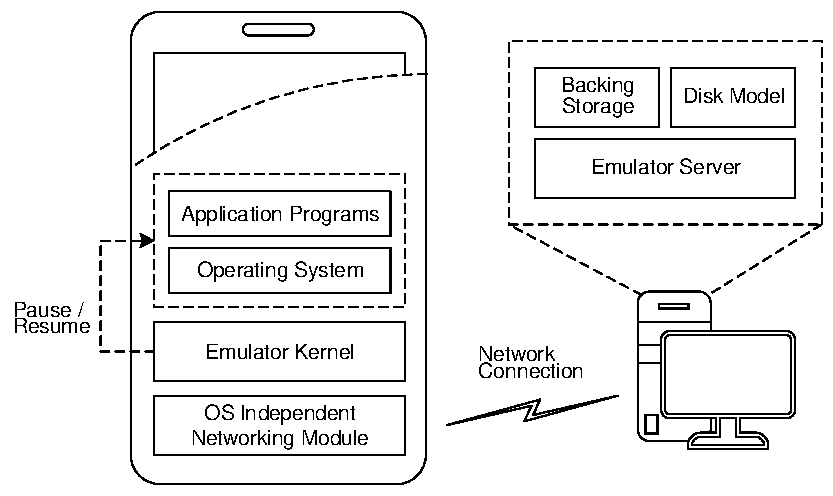
\includegraphics[width=0.9\textwidth]{figures/ch6-emulator-overview.pdf}
	\caption{\label{fig:ch6-emulator-overview}An overview of the proposed storage device emulator.}
\end{figure}

\begin{itemize}
	\item By pausing the state of the OS as necessary whenever the storage device is being emulated, the proposed storage device emulator can overcome the real-time timing constraints faced by emulators which are based on the conventional designs. This allows the proposed emulator to emulate storage devices that would be challenging or even impossible for the conventional storage device emulators. For example, the proposed emulator can allow disk models of arbitrary complexity to be used for simulating the behavior of the target storage device. Another problem with the conventional storage device emulation designs is that the backing storage must be faster than the storage device being emulated. In reality, faster storage devices tend to be more expensive and smaller in size. With the proposed storage device emulator, because the state of the OS is paused while the emulator is accessing the backing storage, slower storage devices can be used as the backing storage for emulating faster storage devices. For example, it is possible to use a slower conventional hard disk drive as the backing storage for emulating fast SSD devices that would otherwise be too large to fit into RAM.
	
	\item Unlike the complete machine simulation approach, there is no need to construct a complete machine simulation model for experimentation. Because the OS and the application programs are run directly on the native machine hardware, the detailed behaviors of the target machine hardware, such as the memory and cache hierarchies, the bandwidth and latencies of the system bus interconnects, and the micro-architecture of the CPU, can automatically be taken into account. Note that because the emulator kernel is also run on the target system's CPU, the cache state of the CPU might be affected. To minimize the disturbances that the proposed emulator might cause to the target system, the data buffers used by the proposed emulator can be allocated from non-cached memory regions. It is also worth noting that because of the way that the state of the OS is paused, the proposed storage device emulator also works with multiprocessor systems.
	
	\item The task of disk model simulation and actual data persistency is done by an emulator server running on a separate computer. This minimizes the interferences that the storage device emulator might cause to the target system. For example, the system memory of the target system does not need to be reserved for use as the backing storage. While it is possible to simulate the disk model directly on the target system while the OS is paused, simulating the disk model on a separate computer can reduce interfering with the cache localities of the target system.
	
	\item Network connection is used as the communication channel between the emulator kernel and the emulator server. Therefore, the features that can be supported by the emulated storage devices will not be limited by the actual I/O interface available on the target system. Furthermore, because the state of the OS is paused while the communications between the emulator kernel and emulator server are taking place, the reading and writing of the actual data for the emulated storage device can take as long as they are required to be transferred over the network channel. For example, for a read operation, the emulator kernel will complete the reading of the actual data of the I/O response from the emulator server before resuming the OS to the running state. This means that the bandwidth of the emulated storage device as perceived by the OS can exceed the bandwidth of the network channel being used. For example, it is possible to emulate storage devices that have transfer rates of over 100MB/s using a physical 802.11b wireless link, which only has a maximum transfer rate of 11Mbps. Moreover, the evaluation results will not be affected by the latencies and jitters of the network communication channel because all data transfers are carried out while the OS is in the paused state.
\end{itemize}

Table~\ref{tab:ch6-1} gives a summary of when and how the proposed storage device emulator could be advantageous compared to the other approaches.

\begin{table}[htbp]%
	\renewcommand{\arraystretch}{1.3}
	\centering
	\caption{Comparison of the proposed approach to the other approaches}\label{tab:ch6-1}
	\noindent\begin{tabularx}{\textwidth}{|p{2.8cm}|p{5.4cm}|X|}
		\hline
		\centering\bfseries Compared to & \centering\bfseries Possible Problems with the Other Approaches & \centering\bfseries\arraybackslash Advantages of the Proposed Approach \\ \hline
		
		\hyphenpenalty=10000\raggedright Complete machine simulation & The fidelity of the complete machine simulation model might not be a good approximation of the target system due to lack of exact models for critical SoC components. \newline\newline
		The speed of the complete machine simulation model might be too slow for conducting large full-system benchmarks. &
		By conducting the experiments using the real hardware of the target system, good system model fidelity and fast simulation speed can be achieved. \\ \hline
		
		\hyphenpenalty=10000\raggedright Conventional real-time storage device emulation &
		The time needed for simulating the disk model might be longer than the desired I/O response timings. \newline\newline
		The speed of the backing storage might be slower than the desired I/O response timings. &
		By pausing the state of the OS while the disk model is being simulated and the backing storage is being accessed, the proposed storage device emulator can spend as long as it requires on preparing the I/O responses. \\ \hline
		
		\hyphenpenalty=10000\raggedright Local virtual storage device emulation &
		The main memory available on the target system might be too small for emulating larger storage devices. &
		By offloading the emulation task to a separate remote server, the size of the emulated storage device can be as large as the backing storage available on the remote server. \\ \hline
		
		\hyphenpenalty=10000\raggedright Remote actual storage device emulation &
		The physical I/O interface available on the target system might not be fast enough (in terms of bandwidth and latency) for emulating the desired storage device. &
		By pausing the OS and transferring the actual data over the network links, storage devices of any speed can be simulated and made available to the OS. \\ \hline
		\end{tabularx}
\end{table}%

The design of the proposed storage device emulator is discussed in the following sections. In section~\ref{sec:ch6-6.1}, the concept of OS state pausing in the context of the proposed storage device emulator is explained. Section~\ref{sec:ch6-6.2} gives an overview of how OS state pausing is utilized in the proposed storage device emulator. Section~\ref{sec:ch6-6.3} describes the emulator server and explains the concept of disk model simulation time rollback, which is required for emulating storage devices that can support concurrent I/O request processing and I/O request prioritization. The detailed operation of the proposed storage device emulator is presented in section~\ref{sec:ch6-6.4}, and finally, the OS independent network subsystem is discussed in section~\ref{sec:ch6-6.5}.

\section{Operating System State Pausing}
\label{sec:ch6-6.1}

The state of the OS can be viewed as composed of the combined state of all the processes running in the OS and the current values in the clock counter and the hardware timers used by the OS. By freezing the execution of all the processes in the OS and stopping the clock counter and the hardware timers, the state of the OS can be paused. In the proposed storage device emulator, the state of the OS is paused by the emulator kernel using the following procedure:
\begin{enumerate*}[label=(\roman*)]
	\item Stop the clock counter and the hardware timers by programming their control registers.
	\item If the target platform is a symmetric multiprocessor system, use IPIs (inter-processor interrupts) to interrupt all the other CPUs in the system and schedules a high priority busy waiting loop on them. The busy waiting loop will prevent the other CPUs from executing any processes that belongs to the OS.
\end{enumerate*}

The execution of the OS is resumed from the paused state using the following procedure: 
\begin{enumerate*}[label=(\roman*)]
	\item Resume the counting of the clock counter and the hardware timers.
	\item Terminate the busy waiting loops so that all the CPUs will resume to their original work.
\end{enumerate*}
The pausing and resuming of the OS is entirely transparent to the applications running on the OS, and the OS can still correctly service any system calls requested by the applications. Therefore, all user space applications can be run unmodified on the proposed system.

While the OS is in the paused state, the emulator kernel will not be able to utilize certain OS services such as interrupts or timers. Therefore, a polling-based OS independent networking module which does not rely on interrupts or system timers is design for use by the emulator kernel to communicate with the emulator server. The details of the OS independent networking module will be further discussed in section~\ref{sec:ch6-6.5}.

Because of the pausing made to the OS, the system time that the OS observes is no longer linked to the real-world time. Instead, a virtual system time which is derived from the value in the clock counter is observed by the OS. To preserve the original system behavior, all the external events to the OS should be scheduled according to the virtual system time. In the proposed storage device emulator, the only external events that need to be considered are the completion signals from the emulated storage device and the timer interrupts. The design of the proposed storage device emulator makes sure that the response signals from the emulated storage device are delivered to the OS according to the virtual system time.

In the ideal case, the state of the OS right before being paused and right after being resumed should be exactly the same. However, there are three factors which can affect the deviation of the OS states before and after pausing:

\begin{itemize}
	\item The first factor is the resolutions of the clock counter and the hardware timers. Each time that the counting of the clock counter and the hardware timers are paused and then resumed, the fraction values that are currently accumulated in the digital circuits will be lost. For example, if the clock counter has a resolution of 1\si{\micro\second}, then any passage of time that is less than 1\si{\micro\second} will be lost when the clock counter is paused by writing to its control registers. In our experimental environment, the resolutions of the clock counter and the hardware timers used by the Linux OS is approximately 3\si{\nano\second}.
	
	\item The second factor is how fast the other CPUs in the system can be put into the busy waiting loop. In the ideal case, the other CPUs in the system should be switched immediately to execute the busy waiting loop as soon as the clock counter and the hardware timers are paused. However, it is possible that the other CPUs in the system will have their interrupts disabled when the IPIs are issued. In this case, the busy waiting loop will have to wait until the interrupts are enabled again. During this period of time, the other CPUs would have completed additional tasks that are not supposed to be done when the OS is in the paused state. On systems that can support non-maskable IPIs, such as the NMI in the x86 processors~\cite{Intel:2013} or the FIQ in the ARM processors, the non-maskable IPIs can be used to immediately put the other CPUs into the busy waiting loop regardless of their interrupt enabling states. In practice, the CPUs in a properly designed system should not be in the interrupt-disabled state for any long periods of time.
	
	\item The third factor is the effect of the CPU cache disturbance. When the OS is in the paused state, the CPU of the target system will need to execute instructions for handling the communication between the emulator kernel and the emulator server, and therefore the cache state of the CPU will be different before and after OS pausing. To get an ideal of the scale of the disturbance that the proposed emulator will have on the target system's CPU cache states, we used the \textit{ftrace}~\cite{Kernel:2014} function tracer in the Linux kernel to trace the kernel execution path for handling I/O requests. With the proposed emulator emulating a virtual storage device, the sizes of instruction codes executed by the CPU for handling a read or write request from user space is approximately 101KB and 151KB, respectively. Compared to a simple local storage device emulation type emulator, the sizes of instruction codes executed by the CPU for handling a read or write request is approximately 91KB and 140KB, respectively. Since the L2 cache size of the CPU used in our experimental platform is 512KB, the additional cache overhead introduced by the proposed emulator is only less than 2\% of the L2 cache. Furthermore, modern embedded processors are likely to have larger caches. For example, the Apple A7 SoC~\cite{wiki:2015:A7} incorporates a 1MB L2 cache and a 4MB L3 cache. The cache disturbance that the proposed emulator will have on those processors would be even less.
\end{itemize}

Even though there could be some slight deviations of the OS states before and after pausing, if the scale of the deviations is small compared to the frequency of its occurrence, then the overall system behavior would still be close enough to the original target system for conducting performance studies. In the proposed emulator, the frequency that the OS state pausing is happening is roughly proportional to the frequency that the I/O requests are processed by the emulated storage device. The scale of the deviation of our experimental platform is at the nanoseconds level, and from the experimental results, we have validated that the proposed OS state pausing approach is effective for emulating storage devices that have service times at the millisecond and microsecond levels.

\section{Operating System State Pausing and Storage Device Emulation}
\label{sec:ch6-6.2}

This section discusses how OS state pausing is utilized in the proposed storage device emulator. During operation, the OS in the proposed storage device emulator is either in the paused state or in the running state. To avoid having a real-time timing constraint on the progressing speed of the emulator server and the performance of the communication channel between the emulator kernel and the emulator server, the emulator kernel is designed to only make requests to the emulator server when the OS is in the paused state. The OS will be put into the paused state whenever the emulator kernel is waiting for the responses from the emulator server for the information that it needs for emulating the storage device. That is, the OS and the emulator server will never be in the operating state at the same time. In other words, the synchronization between the emulator kernel and the emulator server only happens when the OS is in the paused state.

Before resuming the OS back to the running state, the emulator kernel will need to have all the information that it needs for emulating the storage device until the next time point that it will communicate with the emulator server. To achieve this, the emulator server is designed to simulate the disk model to a future time point at which the information of the next I/O response can be determined while the OS is in the paused state.

When the OS is put back to the running state, the emulator kernel will use the information provided by the emulator server to set a timer interrupt at the completion time of the next I/O response. Because the timer service provided by the OS is utilized, the completion times of the I/O responses will automatically be scheduled according to the virtual system time of the OS. When the emulator kernel is notified by the timer interrupt, the corresponding I/O response will then be replied to the OS at the desired completion time as indicated by the disk model.

\begin{figure}[htpb]
	\centering
	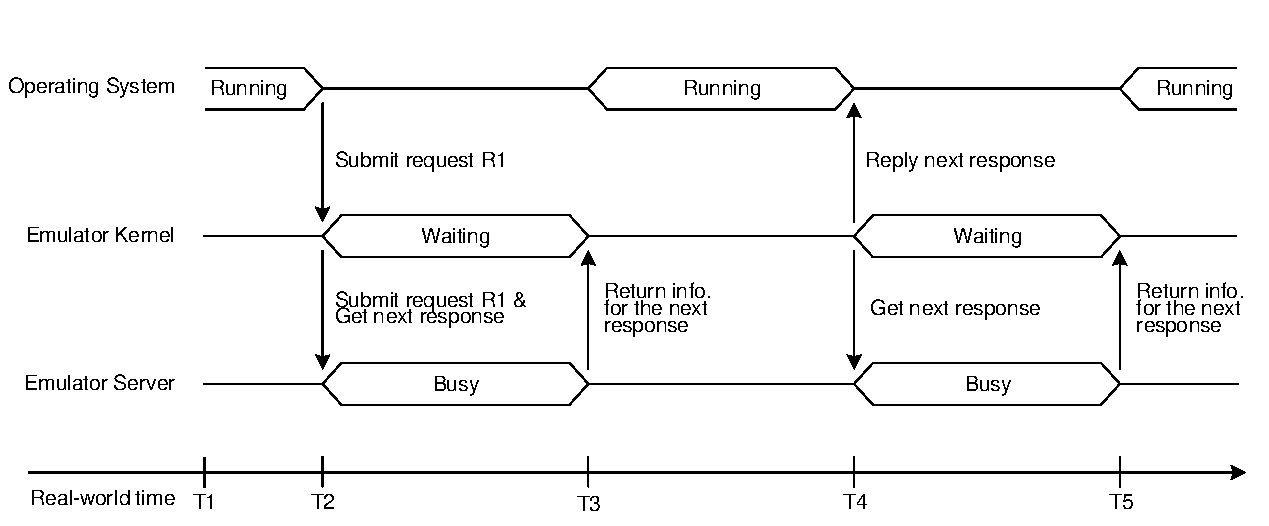
\includegraphics[width=\textwidth]{figures/ch6-fig-6.pdf}
	\caption{\label{fig:ch6-fig-6}Interactions between the OS, the emulator kernel, and the emulator server.}
\end{figure}

A sequence diagram is illustrated in Figure~\ref{fig:ch6-fig-6} to show an example interaction between the OS, the emulator kernel, and the emulator server. As previously shown in Figure~\ref{fig:ch6-emulator-overview}, the emulator kernel is run on the same machine as the OS and the emulator server is run on a separate computer.

At T1, the OS is running continuously and the emulator server is in the idle mode waiting for commands from the emulator kernel. AT T2, an I/O request, R1, is generated by the OS. As soon as R1 is received, the emulator kernel will pause the state of the OS and submit the parameters about R1 to the emulator server. The actual data of R1 is also submitted to or retrieved from the emulator server depending on whether R1 is a read or a write request.

After submitting the I/O request R1, the information for the next I/O response is requested by the emulator kernel. The information of an I/O response includes the ID and the completion time of the I/O response. Because the OS is paused while the emulator server is processing the commands from the emulator kernel, the time between T2 and T3 can be arbitrary long. Before resuming the execution of the OS at T3, the emulator kernel will set a timer event to interrupt itself at the corresponding completion time of the next I/O response. When woken up by the timer interrupt, the emulator kernel can then reply the next I/O response to the OS.

Notice that the emulator kernel asks for the information for the ``next'' I/O response and not specifically for the information for R1, which is the most recently submitted I/O request. This is because that the next I/O request that will be completed by the emulated storage device might not be R1. For example, if the emulated storage device supports I/O prioritization and that it is currently servicing an I/O request that has a higher priority than R1, then R1 will not be serviced until the previous I/O request has been completed. Another example is that if the emulated storage device supports processing of concurrent I/O requests and that there is an I/O request, for example R0, which is currently being processed, then it is possible that R0 will be completed before R1.

Please note that as far as the emulator kernel is concerned, it does not need to know the reason of why the ``next'' I/O response is different from the most recently submitted I/O request. The important thing is that the interface between the emulator kernel and the emulator server will permit the emulator server to change the answer for the next I/O response due to I/O requests that are later submitted to the emulator server.

After the I/O response is replied to the OS at T4, the emulator kernel will communicate with the emulator server again to determine if there will be another I/O response that is going to be completed by the emulated storage device. If there is, then the emulator kernel will set a timer event to interrupt itself at the corresponding completion time of that next I/O response. On the other hand, if there is no further I/O response from the emulated storage device, then the emulator kernel will leave the OS in the running state until future I/O requests are generated by the OS.

\section{Emulator Server with Disk Model Simulation Time Rollback Support}
\label{sec:ch6-6.3}

The emulator server is responsible for simulating the disk model and persisting the actual data for the emulated storage device. It is designed to handle four types of commands from the emulator kernel, which are described in Table II.

\begin{table}[htbp]%
	\renewcommand{\arraystretch}{1.3}
	\centering
	\caption{Commands supported by the emulator server}\label{tab:ch6-2}
	\noindent\begin{tabulary}{\dimexpr\textwidth-3.5cm}{|p{3.5cm}|L|J|}
		\hline
		\centering\bfseries Command Type & \centering\bfseries Parameters & \centering\bfseries\arraybackslash Description \\ \hline
		
		\textit{Reset} &
		\textit{Disk size},\vspace{0.5em}\newline
		\textit{Backing storage configuration},\vspace{0.5em}\newline
		\textit{Disk model configuration} &
		The \textit{reset} command initializes the state of the emulator server to prepare for emulating a new storage device. The \textit{disk size} parameter specifies the size of the storage device to be emulated. The \textit{backing storage configuration} is used for selecting the backing storage device to use (for example, RAM or SSD). The characteristics of the target storage device to be emulated can be controlled by the disk model configuration. For example, the disk model in our experimental implementation can support the configuration of \textit{speedup factor} and the \textit{number of channels}. \\ \hline
		
		\textit{Data Transfer} &
		\textit{Sector number},\vspace{0.5em}\newline
		\textit{Read/write type},\vspace{0.5em}\newline
		\textit{Sector data} &
		The \textit{data transfer} commands are used for the persistence of the actual data. The write data transfer command is used to save the actual data to the backing storage, and the read data transfer command is used for retrieving the actual data from the backing storage. \\ \hline
		
		\textit{Submit Request} &
		\textit{Request time},\vspace{0.5em}\newline
		\textit{Start sector},\vspace{0.5em}\newline
		\textit{Sector count},\vspace{0.5em}\newline
		\textit{Read/write type} &
		The \textit{submit request} command is used for submitting I/O requests to the emulator server. The emulator server will keep track of the I/O requests that have been received and it will simulate the disk model accordingly.\\ \hline
		
		\textit{Get Next Response} &
		\textit{OS system time} &
		The emulator kernel uses the \textit{get next response} command to get the information for the next I/O response that will be completed by the emulated storage device. If there are no I/O requests being processed by the emulated storage device, then the return value of this command will indicate that there will be no next response. \\ \hline
	\end{tabulary}
\end{table}%


In order to support the \textit{get next response} command, the emulator server will need to simulate the disk model past the current system time of the OS. When simulating the disk model between the current system time of the OS and until the completion time of the next I/O response, the disk model is simulated under the assumption that the OS will not submit any additional I/O requests to the emulated storage during this period of time. For example, if an I/O request is submitted to the emulator server at V1 and the next I/O response is determined to be completed at V3, then the disk model is simulated under the assumption that the OS will not submit any I/O request to the emulated storage device between V1 and V3. This assumption is required because the disk model is being simulated into the ``future'' time. However, this assumption might not always be true if the emulated storage device can handle more than one I/O requests from the OS. For example, if another I/O request is generated by the OS between V1 and V3, then the state of the disk model will need to be \textit{rolled back} to a prior simulation time at which when the new I/O request is generated. The disk model can then be simulated again with the new I/O request being taken into account.

\begin{figure}[htpb]
	\centering
	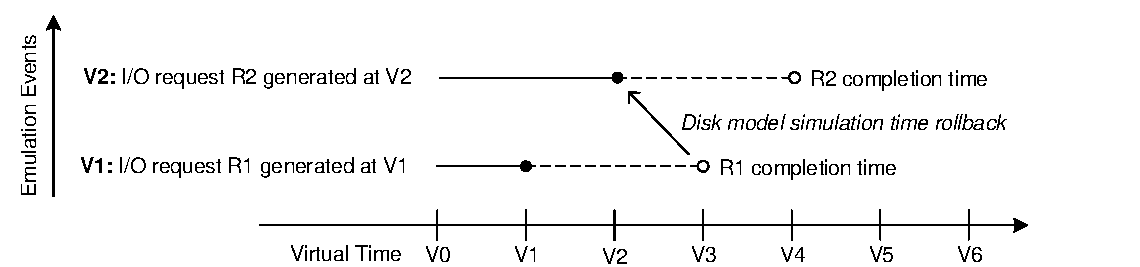
\includegraphics[width=\textwidth]{figures/ch6-fig-7.pdf}
	\caption[Disk model simulation time rollback.]{\label{fig:ch6-fig-7}A scenario showing the emulator server performs a disk model simulation time rollback. Solid circles represent the virtual system time of the OS and white circles represent the simulation time of the disk model.}
\end{figure}

An example is illustrated in Figure~\ref{fig:ch6-fig-7} to show a scenario when disk model simulation time rollback is performed by the emulator server. At virtual time V1, an I/O request, R1 is generated by the OS. Assume that R1 is the only I/O request currently submitted to the emulated storage device and that R1 will be completed by V3 if the emulated storage device does not receive any other I/O requests before V3. When the \textit{get next response} command is issued to the emulator server at V1, the disk model will be simulated to until time V3, at which it is the time that R1 will be completed. The emulator kernel will use the replied information to set a timer to be expired at V3 so that R1 will be replied to the OS when the system time of the OS reaches V3. After setting the timer, the emulator kernel will put the OS back into the running state. Now, assume that the OS has generated another I/O request, R2, when the system time reaches V2. The emulator kernel will then submit R2 to the emulator server and issue another \textit{get next response} command. At this time, the simulation time of the disk model will need to be rolled back to V2 so that I/O request R2 can be properly considered by the disk model.

For example, if R2 has a higher priority than R1, then after the disk model is rolled back to V2, the disk model will determine that the processing of R1 should be preempted by R2. Therefore, when the emulator kernel issues a \textit{get next request} command at V2, the emulator server will reply that the next I/O response is R2. For another example, if the emulated storage device supports concurrent I/O request processing and that R2 has a shorter service time than R1, then even that R2 is received after R1, its completion time might still be earlier than V3. In this case, even if the processing of R1 is not interrupted by R2, the next I/O request that will be completed by the emulated storage device will still change to R2.

In the actual implementation of the emulator server and the disk model, the simulation time of the disk model might not be able to be rolled back to any arbitrary point of time. To allow the rollback of the disk model to any arbitrary point of time would require that every state progression of the disk model to be saved, which might not be practical. A design technique can be used so that the state of the disk model is only saved at the time point at which the \textit{get next response} command is received. With this design technique, the simulation time of the disk model is first rolled back to the previous state at which the previous \textit{get next response} command is issued, and the disk model can then be simulated from there on. Using the scenario illustrated in Figure~\ref{fig:ch6-fig-7} as an example: when the \textit{get next response} command is received at V2, the disk model is rolled back from V3 to V1 and then simulated starting from V1. Between V1 and V2, the disk model will only consider R1. And from V2 and on, the disk model will consider both R1 and R2. With this design technique, supporting disk model simulation time rollback would only require that the emulator server to be able to roll back the disk model to the states at which the previous \textit{get next response} commands are received. This can greatly simplify the design and implementation of the emulator server and the disk model.

For each rollback operation, the amount of work that is discarded is approximately equal to the amount of time for simulating one I/O request. For example, if on average it takes the disk model T units of time to simulate an I/O request, then the cost of each rollback operation, which equals to the discarded simulation progress of the disk model, will be approximately T units of time.

The upper bound for the frequency at which the rollback operations will be occurring during simulation is no more than the number of I/O requests being submitted to the emulator server. For each I/O request submitted to the emulator server, at most one rollback operation could be triggered. That is, if the submission time of the I/O request is earlier than the earliest completion time of the I/O requests already in the disk model, then one rollback operation will be performed on the disk model. Therefore, for N I/O requests, the maximum number of rollback operations that could have occurred will not exceed N.
\section{Detailed Operation of the Proposed Storage Device Emulator}
\label{sec:ch6-6.4}

\begin{figure}[htpb]
	\centering
	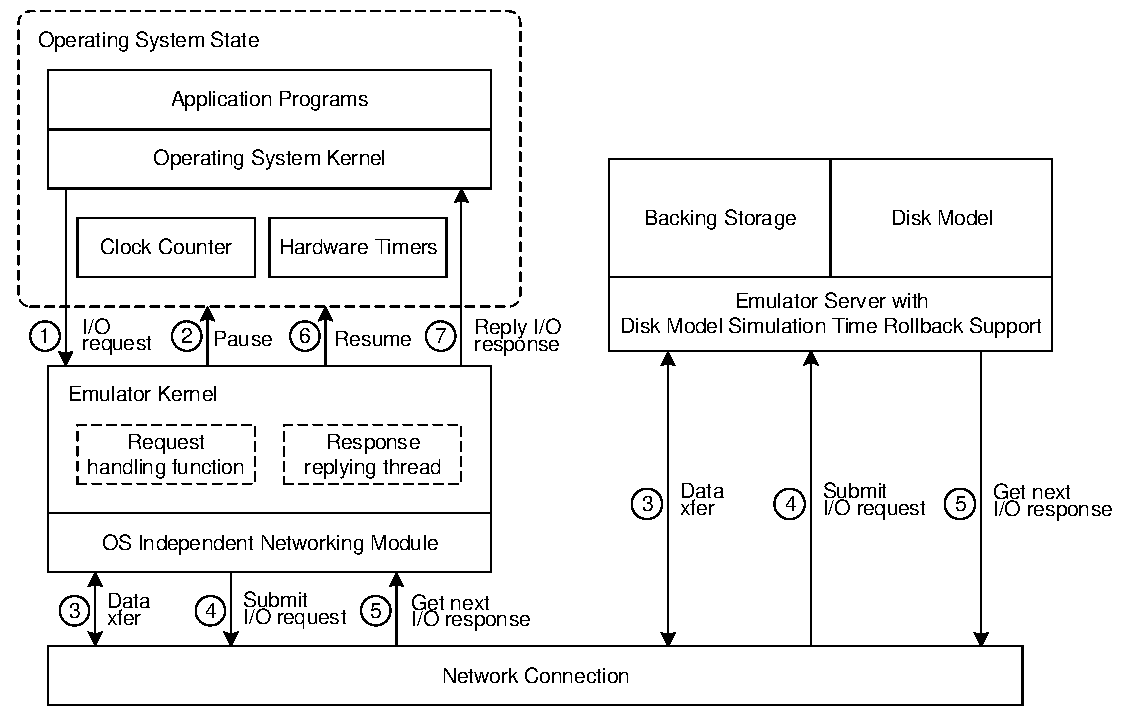
\includegraphics[width=\textwidth]{figures/ch6-fig-8.pdf}
	\caption{\label{fig:ch6-fig-8}Detailed operation of the proposed storage device emulator.}
\end{figure}

A more detailed view of the proposed storage device emulator is illustrated in Figure~\ref{fig:ch6-fig-8}. The emulator kernel is responsible for emulating a virtual storage device to the OS at the block device driver level and is composed of two primary components: the request handling function, (described in algorithm listing~\ref{alg:request-handling-function}) and the response replying thread (described in algorithm listing~\ref{alg:response-replying-thread}). The request handling function is part of the block device driver that is registered to the OS. Whenever the OS generates I/O requests towards the emulated storage device, it will invoke the request processing function.

The response replying thread is a high priority background kernel thread used for replying the I/O responses to the OS. When the completion time of an I/O response is determined, the emulator kernel will set a timer event which will wake up the response replying thread at the corresponding completion time. When the response replying thread is woken up, it will then reply the I/O response to the OS.

The detailed operation steps of the proposed storage device emulator depicted in Figure~\ref{fig:ch6-fig-8} are discussed as follows.

\begin{description}
	\item[Step 1:] Receive I/O request from the OS. When an I/O request is generated by the OS, the request handling function in the emulator kernel will be invoked. A set of non-cacheable memory buffers in the emulator kernel are used to simulate the memory mapped I/O interface of the storage device controller. If the I/O request from the OS is a write request, then the actual data will be copied to the write buffer (the \textit{tempWriteBuffer} in the algorithm listings) of the emulator kernel at this time to mimic the transferring of the actual data to the storage device controller.
	
	\item[Step 2:] Pause the state of the OS. The state of the OS will be paused by the emulator kernel before initiating communication to the emulator server. This allows the emulator server to take as long as it requires for processing the commands from the emulator kernel without affecting the behavior of the emulated storage device as perceived by the OS.
	
	\item[Step 3:] Transfer the actual data of the I/O request. If the I/O request is a write request, then the data that was copied to the write buffer (\textit{tempWriteBuffer}) in step 1 will be transferred to the emulator server for persistence. Otherwise, if the I/O request is a read request, then the actual data of the I/O request will be retrieved from the emulator server and stored in the non-cacheable read buffer (the \textit{tempReadBuffer} in the algorithm listings) of the emulator kernel. The retrieved actual data is not copied directly to the I/O response buffers that belong to the OS at this time to mimic the behavior of real storage devices. For real storage devices, the requested actual data will not be available until the I/O request is completed. If the actual data is copied to the I/O response buffers that belong to the OS at this time, then the temporal cache locality of the actual data will be different from that of the real-world cases. The retrieved actual data will temporarily wait in the read buffer until the I/O response is actually going to be replied to the OS in step 7. At that time, the actual data will then be copied from the read buffer to the I/O response buffers that belong to the OS.
	
	\item[Step 4:] Submit the I/O request to the emulator server. The parameters of the I/O request, which includes the request time, request type (read or write), start sector, and number of sectors, is submitted to the emulator server. These information are used by the disk model to simulate the completion time of the I/O requests.
	
	\item[Step 5:] Get the information of the next I/O response. Before resuming the OS from the paused state, the emulator kernel needs to know the completion time of the next I/O response. A timer event will be set to wake up the response replying thread at the corresponding completion time. If there is a timer event already set for the response replying thread, then the timer event will be updated to the new completion time if it is earlier than the current value set in the timer.
	
	\item[Step 6:] Resume the OS from the paused state. After the response replying thread is properly set to be woken up at the completion time of the next I/O response, the OS will be resumed from the paused state. The OS then runs continuously until one of the two following scenarios happens:
\begin{enumerate*}[label=(\roman*)]
	\item Another I/O request is generated by the OS. In this case, the newly generated I/O request is handled following the same steps beginning from step 1.
	\item The timer event for the response reply thread expires and the response replying thread is woken up. In this case, the processing continues to step 7.
\end{enumerate*}	

	\item[Step 7:] Reply the I/O response to the OS. When the system time of the OS has advanced to the completion time of the next I/O response, the response replying thread will be woken up by the timer event. If the I/O response is for a write request, then the response relying thread simply notifies the OS that the write request has been completed. Otherwise, if the I/O response is for a read request, then the actual data in the \textit{tempReadBuffer} will be first copied to the corresponding I/O response buffers that belong to the OS, and then the OS will be notified about the completion of the read request.
\end{description}


\begin{algorithm}
\small
\newcommand*\Let[2]{\State #1 $\gets$ #2}
	\caption{Request Handling Function
		\label{alg:request-handling-function}}
	\begin{algorithmic}[1]
		\Function{request_fn}{}
		\Let{Request}{get next pending request from OS}
		\If{Request is a write request}
			\Let{Request.tempWriteBuffer}{Sector data}
		\EndIf
		\State Pause OS
		\If{Request is a write request}
			\State Transfer Request.tempWriteBuffer to emulator server;
		\Else
			\Let{Request.tempReadBuffer}{Retrieve sector data from emulator server}
		\EndIf
		\Let{HasNextResponse_T, NextResponseTime_T, NextResponses_T}{Emulator server}
		\If{HasNextResponse_T == TRUE and \newline (HasNextResponse == FALSE or NextResponseTime_T < NextResponseTime)} \label{lst1:line:if}
			\Let{HasNextResponse}{TRUE}
			\Let{NextResponseTime}{NextResponseTime_T}\label{lst1:line:assignNextResponseTime}
			\Let{NextResponses}{NextResponses_T}
			\State{Signal the response replying thread}\label{lst1:line:signal}
		\EndIf
		\State Resume OS

		\EndFunction
	\end{algorithmic}
\end{algorithm}

Remarks on algorithm~\ref{alg:request-handling-function}: In Linux, the request handling function is invoked by the kernel whenever there are I/O requests to be submitted to the storage device. Request.tempWriteBuffer is a non-cached memory buffer for temporarily storing the sector data of a write I/O request. Request.tempReadBuffer is a non-cached memory buffer for temporarily storing the sector data of a read I/O request. The temporary buffers are allocated from a non-cached memory address space to simulate what a real device driver would do. That is, the sector data need to be transferred between the CPU and the device controller. The HasNextResponseTemp, NextResponseTimeTemp, and NextResponsesTemp variables store the information regarding the next I/O response from the emulator server. The if clause in line~\ref{lst1:line:if} tests if the completion time of the new next I/O response will be earlier than the current timer interrupt of the response replying thread. If true, then the response replying thread will be signaled so that the timer interrupt can be updated to an earlier time point corresponding to NextResponseTimeTemp. Note that the request handling function only makes requests to the emulator server while the OS is being put into the paused state.

\begin{algorithm}
	\small
	\newcommand*\Let[2]{\State #1 $\gets$ #2}
	\caption{Response Replying Thread
		\label{alg:response-replying-thread}}
	\begin{algorithmic}[1]
		\State{HasNextResponse = FALSE}
		\Repeat
		\If{HasNextResponse == FALSE} \label{lst2:line:startSleep}
			\State{Sleep until being signaled}
		\EndIf \label{lst2:line:endSleep}
		\Repeat \label{lst2:line:startWaitTimeArrive}
			\State{Sleep until NextResponseTime has arrived or being signaled}
		\Until{NextResponseTime has arrived} \label{lst2:line:endWaitTimeArrive}
		\For{each Response in NextResponses} \label{lst2:line:startReply}
			\If{Response is a read response}
				\State Copy Response.tempReadBuffer to the response buffers belonging to the OS
			\EndIf
			\State Reply Response to operating system
		\EndFor \label{lst2:line:endReply}
		\State Pause OS
		\Let{HasNextResponse, NextResponseTime, NextResponses}{Emulator server} \label{lst2:line:getInfo}
		\State Resume OS
		\Until{Storage emulator is stopped}
	\end{algorithmic}
	\bigskip
\end{algorithm}

Remarks on algorithm~\ref{alg:response-replying-thread}: The response replying thread is a high priority background kernel thread responsible for replying the I/O responses to the OS. In line~\ref{lst2:line:startSleep} to~\ref{lst2:line:endSleep}, if there is currently no I/O response pending to be replied to the OS, the response replying thread will go into an infinite sleep until being signaled by line~\ref{lst1:line:signal} of the request handling function. The while loop between line~\ref{lst2:line:startWaitTimeArrive} and~\ref{lst2:line:endWaitTimeArrive} ensures that the timer interrupt which will wake up the response replying thread is set to the most current value assigned by the request handling function (line~\ref{lst1:line:assignNextResponseTime} of the request handling function). Line~\ref{lst2:line:startReply} to~\ref{lst2:line:endReply} replies the I/O response to the OS when the completion time of the I/O request has arrived. After the I/O response has been replied to the OS, line~\ref{lst2:line:getInfo} gets the information for the next I/O response from the emulator server. Note that the response replying thread only makes requests to the emulator server while the OS is put into the paused state.

\section{Operating System Independent Networking Module}
\label{sec:ch6-6.5}

An OS independent networking module is designed in the proposed storage device emulator to be used by the emulator kernel for communicating with the emulator server. The OS independent networking module is used instead of the standard networking stack that comes with the OS because of the following reasons:

\begin{itemize}
	\item While the OS is in the paused state, the CPUs will have their interrupts disabled. The network device drivers that come with the OS cannot be used because they depend on interrupts for working with the network hardware. In the OS independent networking module, a special polling-based network device driver is implemented for working with the network hardware. The special device driver provides its own set of polling-based APIs for use by the emulator kernel.
	
	\item To minimize the interference that the OS independent networking module will have to the original system behavior, the packet buffers which are used by the network hardware are not allocated from the OS kernel. Instead, a packet buffer manager is designed for allocating and reclaiming the packet buffers from a non-cached memory pool owned by the emulator kernel.
	
	\item When the OS is in the paused state, the timer service provided by the OS will not function properly because the clock counter and the hardware timers are stopped. This means that the TCP implementation in the standard OS networking stack will not work because the retransmission timers will not be functioning correctly. In the proposed storage device emulator, the emulator kernel communicates with the emulator server using the UDP protocol. The UDP packets are assembled and parsed by the emulator kernel without going through the full OS networking stack. To transmit a UDP packet, the UDP packet is assembled by the emulator kernel and handed to the special polling-based device driver in the OS independent networking module directly. To receive the response packet, the emulator kernel uses the polling-based API to poll the network hardware repeatedly until the expected packet has arrived. If the expected response packet is not received after a certain number of polling attempts, the request packet will be retransmitted again by the emulator kernel.
\end{itemize}

\section{Experimental Results}
\label{sec:ch6-6.6}

We have implemented the proposed storage device emulator with the Linux OS. The target hardware platform used is the ZedBoard development board~\cite{ZedBoard:2014}. ZedBoard contains a 667MHz dual-core ARM Cortex-A9 MPCore processor and 512MB of DDR3 main memory. The Linux kernel used is based on the kernel version 3.10.0 from the Xilinx source repository~\cite{Xilinx:2014:kernel}. The root file system used is based on the nano build of the Linaro release version 13.11~\cite{Linaro:2014:v13.11nano}. The device driver for the ARM global timer~\cite{Xilinx:2013:Zynq7010} is backported from the mainline kernel~\cite{Kernel:2013:ARMglobalTimer}, and the Linux kernel is configured to use the ARM global counter as its clocksource and clockevent devices~\cite{Stultz:2005} \cite{GleixnerNiehaus:2006} \cite{GleixnerMolnar:2006} \cite{Gleixner:2007}. The ARM global timer runs at half the speed of the ARM processor. At 333MHz, it provides the clocksource and clockevent devices a timing resolution of approximately 3\si{\nano\second}. In other words, the resolution of the clock counter and hardware timers used by the Linux OS is approximately 3\si{\nano\second}. The emulator server is implemented as a user space program on a separate computer running Ubuntu Linux. The host computer for the emulator server is equipped with an Intel Core i5-3210M CPU running at 2.5GHz, 4GB of RAM, and a Seagate Momentus Thin 320GB hard disk drive as the backing storage. ZedBoard is connected to the emulator server using a 1Gbps Ethernet LAN. 

To measure how much disturbance the operations of the proposed emulator (e.g., OS pausing, OS resuming, network communication, etc.) will have to the target system, the simulation results from the proposed emulator are compared to the results from a reference system.

The reference system is an unmodified Linux OS, which runs on the same ZedBoard platform, and has a RAMDISK storage device emulated by a local emulation type emulator. The parameters of the RAMDISK device are designed so that its performances are comparable to UHS-1 SD cards. The same disk model will be used by both the proposed emulator and the reference system. Ideally, the disturbances caused by the operations of the proposed emulator should be low and the evaluation results from the proposed emulator should match closely to the results from the reference system.

The reasons of why a RAMDISK device, which is emulated by a local emulation type emulator, instead of real storage devices is used in the reference system are given as follows:

\begin{itemize}
	\item The structure of the emulator kernel is very similar to how a local emulation type emulator would be implemented. The main differences between the proposed emulator and a local emulation type emulator are the extra steps needed for pausing and resuming the OS and for performing network communications. Using a local emulation type emulator in the reference system allows us to measure how much disturbance the extra operations of the proposed emulator has caused to the target system.
	
	\item In our experience, the work needed for accurate modeling of real storage devices is not trivial. For example, to model the exact behavior of a NAND storage device that contains a Flash Translation Layer (FTL) would require that the firmware of the FTL to be available; otherwise, the exact sector data placement in the emulated storage device will be different from the real device, and this will lead to different I/O response timings. If the behaviors of the real storage device are not modeled exactly, then testing the proposed emulator using an inexact disk model will mean that we will not be able to tell if the inaccuracies are caused by the disturbances of the proposed emulator or the inaccuracy of the disk model.
	
	\item The physical I/O interface on the target platform might limit the performances or characteristics of the real storage devices that can be tested. For example, the SD interface supported by the ZedBoard is at version 2.00, which can only support a maximum bus speed of 25MB/s. Therefore, it is not possible to validate the proposed emulator with a real SD device faster than 25MB/s on the ZedBoard platform. With a local emulation type emulator, we were able to emulate storage devices that have speeds of over 100MB/s for validating the proposed storage device emulator, which will not be possible if real storage devices are used. Moreover, next generation standards, such as the JEDEC Universal Flash Storage (UFS), will support the command queuing feature, and therefore cannot be emulated over the SD interface. By comparing against a local emulation type emulator, we were able to validate the proposed emulator under concurrent I/O scenarios.
	
	\item Besides using different I/O workloads for testing the proposed storage device emulator, we also want to test if the proposed emulator can handle storage devices of different speeds and concurrency levels. By using a local emulation type emulator as the comparison target, storage devices of different speeds and concurrency levels can easily be modeled for testing.
\end{itemize}
 
\begin{table}[htbp]%
	\centering
	\caption{Performance numbers used for the baseline storage device}\label{tab:ch6-3}
	\noindent\begin{tabular}{lcccc}
		\toprule
		& \multicolumn{2}{c}{Random Workload} & \multicolumn{2}{c}{Sequential Workload} \\
		\cmidrule(lr){2-3}
		\cmidrule(lr){4-5}
		\parbox{3cm}{\centering Transfer size} & \parbox{2cm}{\centering Read (\si{\milli\second}) } & \parbox{2cm}{\centering Write (\si{\milli\second}) } & \parbox{2cm}{\centering Read (\si{\milli\second}) } & \parbox{3cm}{\centering Write (\si{\milli\second})} \\
		
		\midrule
		
		512 bytes & 0.0051 & 1.1136 & 0.0019 & 0.0092 \\
		1 KB & 0.0053 & 1.1123 & 0.0020 & 0.0095 \\
		2 KB & 0.0054 & 1.1136 & 0.0023 & 0.0099 \\
		4 KB & 0.0057 & 1.1601 & 0.0027 & 0.0115 \\
		8 KB & 0.0063 & 1.2853 & 0.0033 & 0.0136 \\
		16 KB & 0.0071 & 1.2579 & 0.0036 & 0.0035 \\
		32 KB & 0.0096 & 2.2222 & 0.0068 & 0.0070 \\
		64 KB & 0.0151 & 2.7027 & 0.0139 & 0.0137 \\
		
		\bottomrule
	\end{tabular}
\end{table}%

The random and sequential read/write performances of a Transcend Ultra High Speed (UHS) Speed Class 1 SD memory card are measured and used to model a hypothetical baseline storage device. The measured performance numbers are shown in Table III. It is important to note that the baseline storage device is by no means trying to simulate the actual behavior of the Transcend SD memory card. These performance numbers are used for modeling the baseline storage device so that the performance of the baseline storage device is in line with the current top of the line storage devices.

The characteristics of the baseline storage device can be controlled by two parameters: the speedup factor and the number of channels parameters. Both parameters are varied from $\times$1 to $\times$4 for deriving a total of 16 storage device configurations for validating the proposed storage device emulator. The storage device configuration ChN-xS means that the number of channels the storage device has is N and it has a speedup factor of S. The number of channels parameter configures the number of concurrent I/O requests that the storage device can process simultaneously. For example, if four I/O requests are submitted to an emulated storage device which has four channels, then all four I/O requests will be processed concurrently. The speedup factor parameter configures how much faster the storage device is compared to the baseline storage device. For example, a speedup factor of two means that the response times of the emulated storage device will be half of the baseline storage device.

The total amount of memory available on ZedBoard is only 512MB. Therefore, the size of the emulated storage device is set to be 400MB, which leaves 112MB of memory for use by the Linux OS. A 12MB tmpfs temporary file storage is created and used for temporarily storing the outputs from the benchmark applications. Note that for the proposed storage emulator, because the actual data is persisted on the remote host, the Linux OS will be able to use the complete 512MB of main memory. However, we still configure the Linux OS to use only 112MB of memory so that the testing conditions are equivalent to the reference system.

The benchmarks are executed using the auto-pilot automation framework~\cite{Wright:2005:auto-pilot} \cite{Wright:2007:auto-pilot}. Each benchmark is run at least 10 times and until the radius of the 95\% confident interval is less than 5\% of the mean. The \textit{cron} and \textit{rsyslog} services in the Linux OS are disabled while the benchmarks are performed to reduce possible interferences. The system is rebooted after each benchmark run. The evaluation results are presented in the following subsections.
	
\subsection{Sequential Read Bandwidth}
\label{sec:ch6-6.6.1}

\begin{table}[htbp]%
	\small
	\begin{center}
	\caption{Sequential read bandwidth}\label{tab:ch6-5}
	\hspace*{-2cm}
	\noindent\begin{tabular}{
			l
			S[table-format=3.2]
			S[table-format=3.2]
			S[table-format=3.2]
			S[table-format=3.2]
			S[table-format=3.2]
			S[table-format=3.2]
			S[table-format=1.2]
			S[table-format=1.2]
			c}
		\toprule
		{Test Config} & {Mean} & {Median} & {Low} & {High} & {Min} & {Max} & {SDEV\%} & {HW\%} & \multicolumn{1}{c}{Diff} \\
		\midrule
		
		Ch1-x1 Ref. & 36.58 & 36.58 & 36.52 & 36.64 & 36.38 & 36.68 & 0.24 & 0.17 &  \\
		Ch1-x1 & 36.48 & 36.48 & 36.45 & 36.51 & 36.42 & 36.54 & 0.12 & 0.09 & -0.26\% \\
		Ch1-x2 Ref. & 61.74 & 61.82 & 61.61 & 61.87 & 61.42 & 61.97 & 0.29 & 0.21 & \\
		Ch1-x2 & 61.49 & 61.50 & 61.40 & 61.57 & 61.23 & 61.67 & 0.19 & 0.14 & -0.41\% \\
		Ch1-x3 Ref. & 80.07 & 80.07 & 79.89 & 80.26 & 79.64 & 80.46 & 0.33 & 0.23 & \\
		Ch1-x3 & 79.51 & 79.47 & 79.40 & 79.61 & 79.27 & 79.74 & 0.19 & 0.13 & -0.70\%\\
		Ch1-x4 Ref. & 93.55 & 93.67 & 93.22 & 93.89 & 92.56 & 94.04 & 0.51 & 0.36 & \\
		Ch1-x4 & 93.04 & 92.99 & 92.85 & 93.24 & 92.66 & 93.44 & 0.29 & 0.21 & -0.55\% \\
		Ch2-x1 Ref. & 63.41 & 63.41 & 63.35 & 63.47 & 63.23 & 63.54 & 0.14 & 0.10 &\\
		Ch2-x1 & 63.17 & 63.20 & 63.09 & 63.25 & 62.97 & 63.30 & 0.18 & 0.13 &-0.38\% \\
		Ch2-x2 Ref. & 97.61 & 97.74 & 97.29 & 97.93 & 96.84 & 98.14 & 0.46 & 0.33 & \\
		Ch2-x2 & 96.96 & 97.06 & 96.66 & 97.25 & 96.18 & 97.40 & 0.43 & 0.31 &-0.67\% \\
		Ch2-x3 Ref. & 117.89 & 117.85 & 117.61 & 118.16 & 117.32 & 118.41 & 0.33 & 0.24 & \\
		Ch2-x3 & 117.01 & 117.11 & 116.63 & 117.39 & 115.97 & 117.69 & 0.45 & 0.32 & -0.74\% \\
		Ch2-x4 Ref. & 128.70 & 128.76 & 127.99 & 129.40 & 126.61 & 130.06 & 0.77 & 0.55 & \\
		Ch2-x4 & 128.37 & 128.70 & 127.04 & 129.69 & 123.70 & 130.62 & 1.44 & 1.03 & -0.26\% \\
		Ch3-x1 Ref. & 85.64 & 85.59 & 85.38 & 85.91 & 85.13 & 86.23 & 0.43 & 0.31 & \\
		Ch3-x1 & 85.99 & 86.02 & 85.73 & 86.25 & 85.33 & 86.38 & 0.42 & 0.30 & 0.41\% \\
		Ch3-x2 Ref. & 111.27 & 111.30 & 110.80 & 111.73 & 110.07 & 112.12 & 0.58 & 0.42 &\\
		Ch3-x2 & 110.72 & 110.80 & 110.26 & 111.19 & 109.33 & 111.70 & 0.59 & 0.42 & -0.49\% \\
		Ch3-x3 Ref. & 125.72 & 125.87 & 125.10 & 126.34 & 124.61 & 126.98 & 0.69 & 0.49 & \\
		Ch3-x3 & 124.89 & 124.95 & 124.32 & 125.46 & 123.64 & 126.07 & 0.64 & 0.46 & -0.66\% \\
		Ch3-x4 Ref. & 131.48 & 131.22 & 130.47 & 132.49 & 129.90 & 134.53 & 1.07 & 0.77 & \\
		Ch3-x4 & 132.16 & 132.25 & 131.56 & 132.76 & 129.98 & 132.97 & 0.64 & 0.45 & 0.52\% \\
		Ch4-x1 Ref. & 84.68 & 84.75 & 84.53 & 84.83 & 84.32 & 84.94 & 0.25 & 0.18 & \\
		Ch4-x1 & 84.67 & 84.61 & 84.51 & 84.84 & 84.37 & 85.04 & 0.27 & 0.20 & 0.01\% \\
		Ch4-x2 Ref. & 110.00 & 109.99 & 109.77 & 110.23 & 109.54 & 110.48 & 0.29 & 0.21 & \\
		Ch4-x2 & 109.60 & 109.66 & 109.19 & 110.01 & 108.84 & 110.41 & 0.52 & 0.37 & -0.36\% \\
		Ch4-x3 Ref. & 121.73 & 121.72 & 121.47 & 122.00 & 121.34 & 122.47 & 0.30 & 0.22 & \\
		Ch4-x3 & 121.27 & 121.41 & 120.92 & 121.62 & 120.57 & 122.11 & 0.40 & 0.29 & -0.38\% \\
		Ch4-x4 Ref. & 131.66 & 131.92 & 129.95 & 133.38 & 126.25 & 134.62 & 1.82 & 1.30 & \\
		Ch4-x4 & 131.92 & 132.53 & 130.77 & 133.07 & 127.88 & 133.31 & 1.22 & 0.87 & 0.20\% \\
			
		\bottomrule
	\end{tabular}
	\hspace*{-2cm}
	\end{center}
	
	Remarks: Units are in MB/s. Low and high are the Student-\textit{t} confidence interval error bar values. SDEV\% and HW\% are the standard deviation and half-width of the confidence interval as a percent of the mean.
\end{table}%

\begin{figure}[htpb]
	\centering
	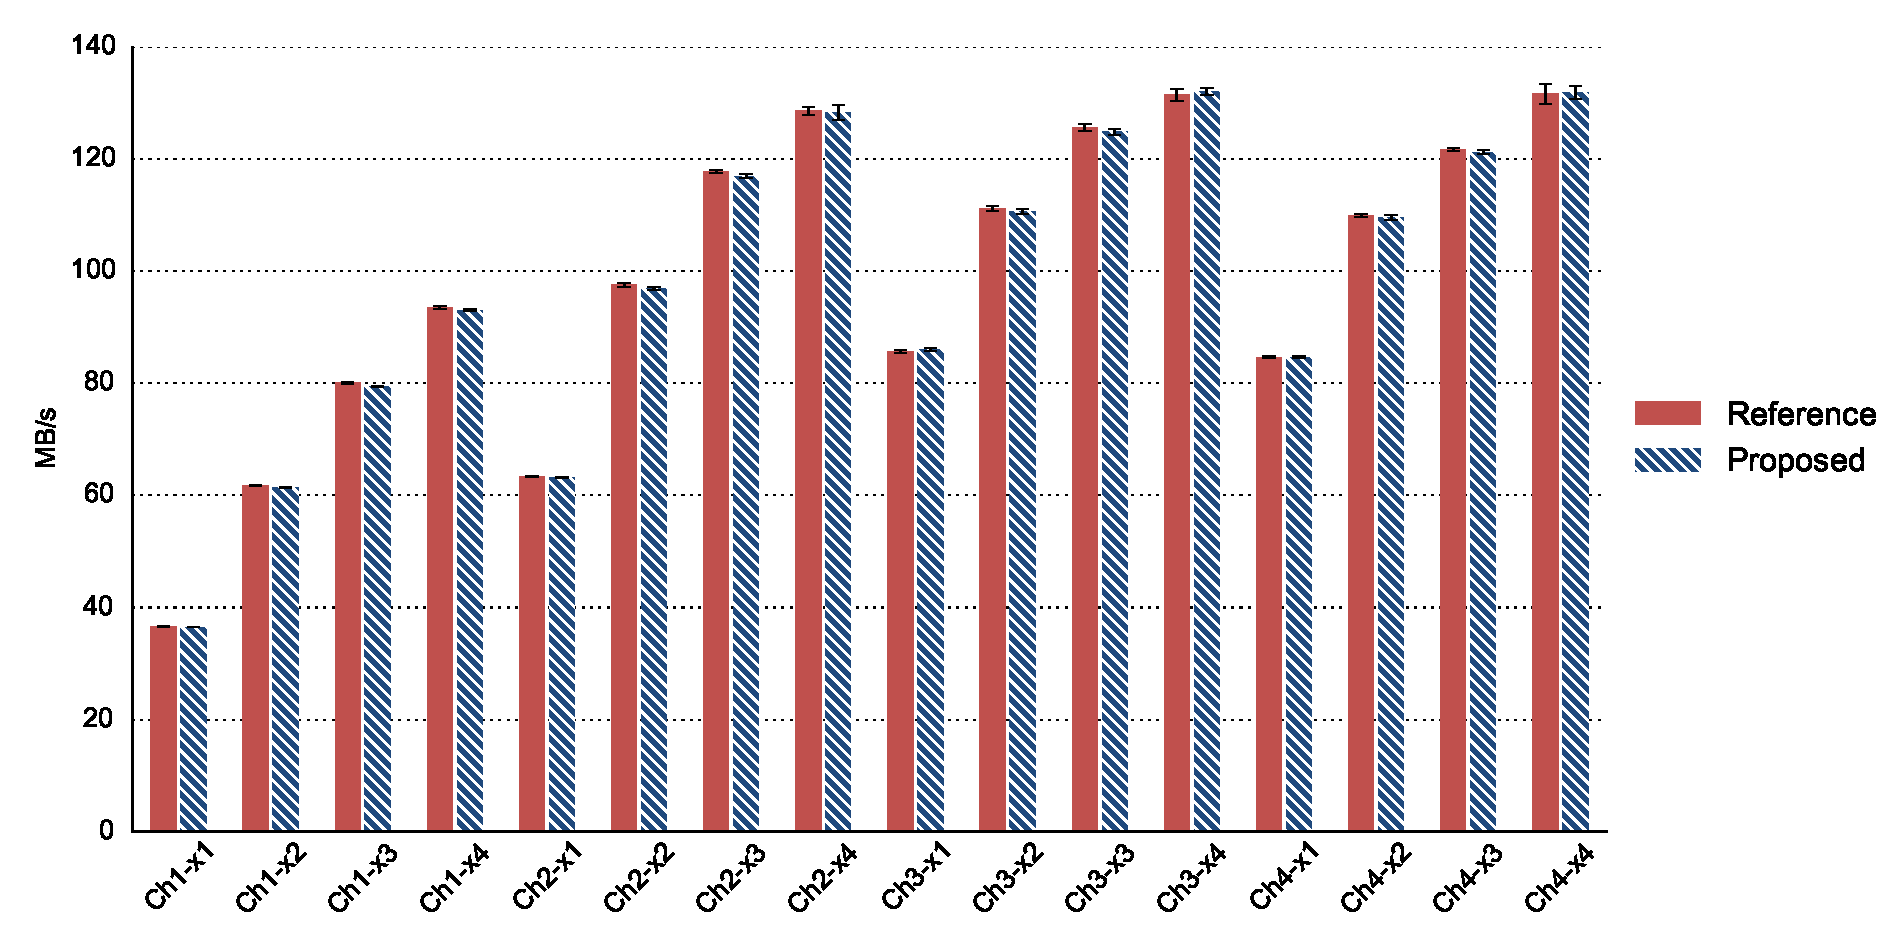
\includegraphics[width=\textwidth]{figures/ch6-fig-9.pdf}
	\caption[Sequential read bandwidth.]{\label{fig:ch6-fig-9}Sequential read bandwidth. Error bars represent the 95\% confidence intervals of the means.}
\end{figure}

\begin{table}[htbp]%
	\centering
	\caption{Frequency of disk model rollback operations for the sequential read workload}\label{tab:ch6-5-rollback}
	\noindent\begin{tabular}{cc}
		\toprule
		Storage device configuration &
		Percentage of I/Os causing rollbacks \\
		\midrule
		Ch1-x1 & 0\% \\
		Ch1-x2 & 0\% \\
		Ch1-x3 & 0\% \\
		Ch1-x4 & 0\% \\
		Ch2-x1 & 49\% \\
		Ch2-x2 & 49\% \\
		Ch2-x3 & 49\% \\
		Ch2-x4 & 49\% \\
		Ch3-x1 & 85\% \\
		Ch3-x2 & 64\% \\
		Ch3-x3 & 63\% \\
		Ch3-x4 & 49\% \\
		Ch4-x1 & 73\% \\
		Ch4-x2 & 74\% \\
		Ch4-x3 & 62\% \\
		Ch4-x4 & 49\% \\
		\bottomrule
	\end{tabular}
\end{table}%

In the first test, the sequential read bandwidth of the emulated storage device is measured using the \textit{hdparm} utility. The I/O scheduler for the emulated storage device is set to the NOOP scheduler. Setting the NOOP I/O scheduler disables the anticipatory I/O scheduling behavior that would otherwise be performed by the default I/O scheduler in the Linux kernel. With anticipatory I/O scheduling disabled, the read requests generated by the \textit{hdparm} utility will be submitted to the emulated storage device as soon as they are created. The measured results are listed in Table~\ref{tab:ch6-5} and graphed in Figure~\ref{fig:ch6-fig-9}. All results from the proposed storage device emulator are within 1\% differences to the results from the reference system. The percentage of all the I/O requests that will cause disk model simulation time rollbacks are listed in Table~\ref{tab:ch6-5-rollback}  


\subsection{The Postmark Benchmark}
\label{sec:ch6-6.6.2}

\begin{table}[htbp]%
	\small
	\begin{center}
	\caption{Elapsed time of the postmark workload}\label{tab:ch6-6}
	\hspace*{-10cm}
	\noindent\begin{tabular}{
			l
			S[table-format=3.3]
			S[table-format=3.3]
			S[table-format=3.3]
			S[table-format=3.3]
			S[table-format=3.3]
			S[table-format=3.3]
			S[table-format=1.2]
			S[table-format=1.2]
			r}
		\toprule
		{Test Config} & {Mean} & {Median} & {Low} & {High} & {Min} & {Max} & {SDEV\%} & {HW\%} & \multicolumn{1}{c}{Diff} \\
		\midrule
		
Ch1-x1 Ref. & 179.866  & 179.670  & 179.327  & 180.406  & 179.375  & 180.416  & 0.24  & 0.30 & \\
Ch1-x1 & 176.830  & 177.071  & 175.859  & 177.802  & 175.797  & 177.778  & 0.44  & 0.55 & -1.69\% \\
Ch1-x2 Ref. & 88.943  & 88.714  & 87.955  & 89.931  & 88.005  & 90.050  & 0.89  & 1.11 & \\
Ch1-x2 & 87.756  & 87.881  & 87.196  & 88.317  & 87.053  & 88.205  & 0.51  & 0.64 & -1.33\% \\
Ch1-x3 Ref. & 58.399  & 58.273  & 57.949  & 58.850  & 58.096  & 58.991  & 0.62  & 0.77 & \\
Ch1-x3 & 57.940  & 58.198  & 57.176  & 58.705  & 56.858  & 58.323  & 1.06  & 1.32 & -0.79\% \\
Ch1-x4 Ref. & 42.136  & 42.130  & 41.809  & 42.462  & 41.770  & 42.514  & 0.63  & 0.78 & \\
Ch1-x4 & 42.322  & 42.224  & 41.894  & 42.750  & 41.903  & 42.738  & 0.82  & 1.01 & 0.44\% \\
Ch2-x1 Ref. & 90.294  & 90.327  & 89.402  & 91.187  & 89.557  & 91.221  & 0.80  & 0.99 & \\
Ch2-x1 & 90.647  & 90.921  & 89.268  & 92.026  & 89.032  & 91.840  & 1.23  & 1.52 & 0.39\% \\
Ch2-x2 Ref. & 44.016  & 43.910  & 43.687  & 44.345  & 43.769  & 44.383  & 0.60  & 0.75 & \\
Ch2-x2 & 43.842  & 43.847  & 43.333  & 44.351  & 43.429  & 44.324  & 0.94  & 1.16 & -0.39\% \\
Ch2-x3 Ref. & 28.287  & 28.243  & 28.128  & 28.447  & 28.156  & 28.481  & 0.45  & 0.56 & \\
Ch2-x3 & 28.313  & 28.311  & 28.111  & 28.516  & 28.110  & 28.488  & 0.58  & 0.72 & 0.09\% \\
Ch2-x4 Ref. & 21.451  & 21.478  & 21.352  & 21.551  & 21.340  & 21.547  & 0.37  & 0.46 & \\
Ch2-x4 & 21.392  & 21.348  & 21.248  & 21.535  & 21.305  & 21.581  & 0.54  & 0.67 & -0.28\% \\
Ch3-x1 Ref. & 60.453  & 60.547  & 59.501  & 61.405  & 59.662  & 61.429  & 1.27  & 1.58 & \\
Ch3-x1 & 60.735  & 60.521  & 60.238  & 61.233  & 60.405  & 61.201  & 0.66  & 0.82 & 0.47\% \\
Ch3-x2 Ref. & 28.839  & 28.881  & 28.497  & 29.180  & 28.533  & 29.163  & 0.95  & 1.18 & \\
Ch3-x2 & 29.006  & 28.935  & 28.812  & 29.199  & 28.900  & 29.273  & 0.54  & 0.67 & 0.58\% \\
Ch3-x3 Ref. & 18.888  & 18.853  & 18.776  & 19.000  & 18.827  & 19.042  & 0.48  & 0.59 & \\
Ch3-x3 & 18.965  & 18.905  & 18.800  & 19.130  & 18.869  & 19.186  & 0.70  & 0.87 & 0.41\% \\
Ch3-x4 Ref. & 14.267  & 14.262  & 14.222  & 14.311  & 14.225  & 14.320  & 0.25  & 0.31 & \\
Ch3-x4 & 14.212  & 14.207  & 14.144  & 14.280  & 14.139  & 14.293  & 0.39  & 0.48 & -0.38\% \\
Ch4-x1 Ref. & 47.027  & 47.050  & 46.817  & 47.236  & 46.808  & 47.198  & 0.36  & 0.45 & \\
Ch4-x1 & 47.005  & 46.949  & 46.504  & 47.506  & 46.471  & 47.444  & 0.86  & 1.07 & -0.05\% \\
Ch4-x2 Ref. & 21.997  & 22.012  & 21.821  & 22.173  & 21.854  & 22.200  & 0.64  & 0.80 & \\
Ch4-x2 & 22.027  & 22.039  & 21.933  & 22.120  & 21.932  & 22.121  & 0.34  & 0.42 & 0.14\% \\
Ch4-x3 Ref. & 14.245  & 14.227  & 14.184  & 14.306  & 14.195  & 14.324  & 0.35  & 0.43 & \\
Ch4-x3 & 14.330  & 14.312  & 14.246  & 14.413  & 14.268  & 14.419  & 0.47  & 0.58 & 0.60\% \\
Ch4-x4 Ref. & 10.809  & 10.807  & 10.760  & 10.859  & 10.762  & 10.850  & 0.37  & 0.46 & \\
Ch4-x4 & 10.806  & 10.821  & 10.711  & 10.902  & 10.689  & 10.900  & 0.71  & 0.88 & -0.03\% \\

		\bottomrule
	\end{tabular}
	\hspace*{-10cm}
	\end{center}
	
	Remarks: Units are in 100 seconds. Low and high are the Student-\textit{t} confidence interval error bar values. SDEV\% and HW\% are the standard deviation and half-width of the confidence interval as a percent of the mean.
\end{table}%



\begin{figure}[htpb]
	\centering
	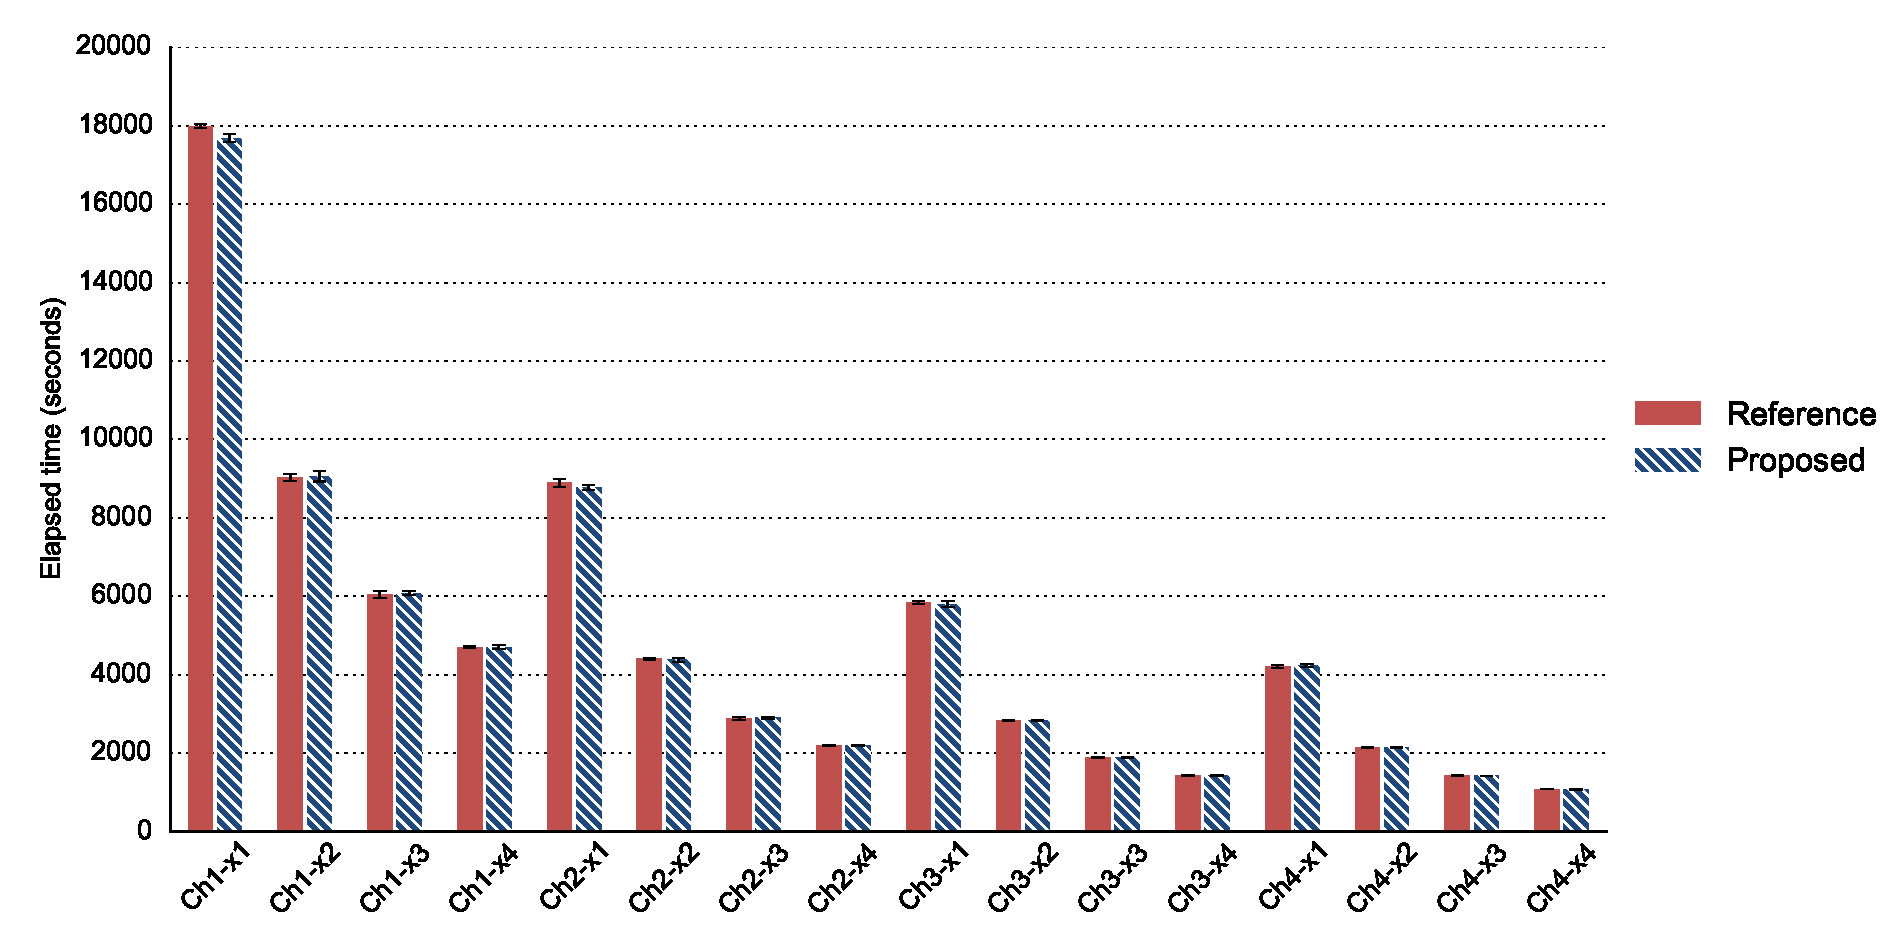
\includegraphics[width=\textwidth]{figures/ch6-fig-10.pdf}
	\caption[Elapsed time of the postmark workload.]{\label{fig:ch6-fig-10}Elapsed time of the postmark workload. Error bars represent the 95\% confidence intervals of the means.}
\end{figure}

\begin{table}[htbp]%
	\centering
	\caption{Frequency of disk model rollback operations for the postmark workload}\label{tab:ch6-6-rollback}
	\noindent\begin{tabular}{cc}
		\toprule
		Storage device configuration &
		Percentage of I/Os causing rollbacks \\
		\midrule
		Ch1-x1 & 0\% \\
		Ch1-x2 & 0\% \\
		Ch1-x3 & 0\% \\
		Ch1-x4 & 0\% \\
		Ch2-x1 & 96\% \\
		Ch2-x2 & 91\% \\
		Ch2-x3 & 87\% \\
		Ch2-x4 & 80\% \\
		Ch3-x1 & 97\% \\
		Ch3-x2 & 91\% \\
		Ch3-x3 & 85\% \\
		Ch3-x4 & 81\% \\
		Ch4-x1 & 95\% \\
		Ch4-x2 & 90\% \\
		Ch4-x3 & 86\% \\
		Ch4-x4 & 81\% \\
		\bottomrule
	\end{tabular}
\end{table}%

The postmark workload is used as the next set of workloads for validation. The ext3 file system is created on the emulated storage device and both scenarios for the NOOP I/O scheduler and the CFQ I/O scheduler are tested. To test how the proposed storage emulator works under multithreaded environment, 8 concurrent postmark threads are used to generate a total of 100,000 transactions over a set of 10,000 files. Each postmark thread will generate 12,500 transactions. All results from the proposed storage device emulator are within 2\% differences to the results from the reference system. The evaluation results for the CFQ I/O scheduler are listed in Table~\ref{tab:ch6-6} and graphed in Figure~\ref{fig:ch6-fig-10}. The percentage of all the I/O requests that will cause disk model simulation time rollbacks are listed in Table~\ref{tab:ch6-6-rollback}  

To give an idea of the I/O patterns generated by the above postmark setup, the the randomness of the generated workloads are measured and listed in Table~\ref{tab:ch6-postmark-randomness}.

\begin{table}[htbp]%
	\centering
	\caption{I/O request randomness of the postmark workload}\label{tab:ch6-postmark-randomness}
	\noindent\begin{tabular}{ccc}
		\toprule
		&\multicolumn{2}{c}{Percentage of random I/O requests}\\
		\cmidrule(lr){2-3}
		\parbox{3cm}{\centering Storage device \\ configuration} &
		\parbox{4cm}{\centering with the CFQ\\I/O scheduler}&
		\parbox{4cm}{\centering with the NOOP\\I/O scheduler}\\
		
		\midrule
		Ch1-x1 & 97.23\% & 96.76\% \\
		Ch1-x2 & 97.26\% & 96.61\% \\
		Ch1-x3 & 96.96\% & 96.83\% \\
		Ch1-x4 & 96.84\% & 96.79\% \\
		Ch2-x1 & 96.07\% & 96.43\% \\
		Ch2-x2 & 96.24\% & 96.27\% \\
		Ch2-x3 & 96.38\% & 96.53\% \\
		Ch2-x4 & 96.36\% & 96.84\% \\
		Ch3-x1 & 95.98\% & 96.46\% \\
		Ch3-x2 & 96.35\% & 96.47\% \\
		Ch3-x3 & 96.56\% & 96.95\% \\
		Ch3-x4 & 96.92\% & 97.20\% \\
		Ch4-x1 & 96.16\% & 96.17\% \\
		Ch4-x2 & 96.35\% & 96.74\% \\
		Ch4-x3 & 96.88\% & 97.15\% \\
		Ch4-x4 & 97.29\% & 97.44\% \\
		\bottomrule
	\end{tabular}
\end{table}%


\subsection{Linux Kernel Source Archive Extraction and Word Count}
\label{sec:ch6-6.6.3}

\begin{table}[htbp]%
	\small
	\begin{center}
	\caption{Elapsed time of Linux kernel source archive extraction and word count}\label{tab:ch6-7}
	\hspace*{-2cm}
	\noindent\begin{tabular}{
			l
			S[table-format=3.2]
			S[table-format=3.2]
			S[table-format=3.2]
			S[table-format=3.2]
			S[table-format=3.2]
			S[table-format=3.2]
			S[table-format=1.2]
			S[table-format=1.2]
			r}
		\toprule
		{Test Config} & {Mean} & {Median} & {Low} & {High} & {Min} & {Max} & {SDEV\%} & {HW\%} & \multicolumn{1}{c}{Diff} \\
		\midrule
		
		Ch1-x1 Ref. & 335.17  & 332.95  & 330.27  & 340.07  & 326.38  & 345.15  & 2.05  & 1.46 & \\
		Ch1-x1 & 328.92  & 326.83  & 322.97  & 334.87  & 318.08  & 340.87  & 2.53  & 1.81 & -1.87\% \\
		Ch1-x2 Ref. & 186.27  & 185.40  & 183.38  & 189.16  & 180.34  & 193.04  & 2.17  & 1.55 & \\
		Ch1-x2 & 188.25  & 188.01  & 184.41  & 192.09  & 181.40  & 196.96  & 2.85  & 2.04 & 1.06\% \\
		Ch1-x3 Ref. & 162.22  & 162.04  & 159.98  & 164.46  & 157.74  & 166.61  & 1.93  & 1.38 & \\
		Ch1-x3 & 162.99  & 162.34  & 161.03  & 164.94  & 160.48  & 169.43  & 1.67  & 1.20 & 0.47\% \\
		Ch1-x4 Ref. & 153.93  & 152.34  & 150.26  & 157.60  & 148.39  & 176.21  & 4.31  & 2.38 & \\
		Ch1-x4 & 152.83  & 152.94  & 151.76  & 153.91  & 150.48  & 155.58  & 0.98  & 0.70 & -0.71\% \\	
		Ch2-x1 Ref. & 184.21  & 184.49  & 181.03  & 187.39  & 177.93  & 189.77  & 2.41  & 1.73 & \\
		Ch2-x1 & 181.93  & 179.86  & 177.68  & 186.19  & 174.86  & 195.40  & 3.68  & 2.34 & -1.24\% \\
		Ch2-x2 Ref. & 154.29  & 154.44  & 152.46  & 156.12  & 150.05  & 158.18  & 1.66  & 1.19  & \\
		Ch2-x2 & 154.92  & 154.82  & 153.40  & 156.43  & 150.73  & 157.40  & 1.37  & 0.98 & 0.41\% \\
		Ch2-x3 Ref. & 147.60  & 147.55  & 146.88  & 148.32  & 145.86  & 149.25  & 0.68  & 0.49 & \\
		Ch2-x3 & 148.38  & 148.30  & 147.79  & 148.97  & 147.47  & 150.30  & 0.56  & 0.40 & 0.53\% \\
		Ch2-x4 Ref. & 145.95  & 145.97  & 145.47  & 146.43  & 145.26  & 147.49  & 0.46  & 0.33 & \\
		Ch2-x4 & 146.22  & 146.18  & 145.62  & 146.82  & 145.01  & 147.74  & 0.58  & 0.41 & 0.18\% \\
		Ch3-x1 Ref. & 171.05  & 171.03  & 166.87  & 175.22  & 163.22  & 186.23  & 3.63  & 2.44 & \\
		Ch3-x1 & 171.69  & 172.34  & 168.09  & 175.29  & 163.12  & 178.03  & 2.93  & 2.10 & 0.38\% \\
		Ch3-x2 Ref. & 152.70  & 152.25  & 151.49  & 153.90  & 150.39  & 155.78  & 1.10  & 0.79 & \\
		Ch3-x2 & 152.44  & 151.74  & 150.93  & 153.95  & 150.13  & 156.69  & 1.38  & 0.99 & -0.17\% \\
		Ch3-x3 Ref. & 146.66  & 146.68  & 146.30  & 147.03  & 145.75  & 147.62  & 0.35  & 0.25 & \\
		Ch3-x3 & 147.15  & 147.37  & 146.64  & 147.67  & 145.63  & 148.05  & 0.49  & 0.35 & 0.33\% \\
		Ch3-x4 Ref. & 145.67  & 145.55  & 145.36  & 145.98  & 144.97  & 146.46  & 0.30  & 0.21 & \\
		Ch3-x4 & 145.52  & 145.37  & 145.30  & 145.74  & 145.21  & 146.00  & 0.21  & 0.15 & -0.10\% \\
		Ch4-x1 Ref. & 168.66  & 167.48  & 166.15  & 171.17  & 164.61  & 175.39  & 2.08  & 1.49 & \\
		Ch4-x1 & 166.84  & 167.60  & 164.74  & 168.94  & 162.15  & 171.77  & 1.76  & 1.26 & -1.08\% \\
		Ch4-x2 Ref. & 151.06  & 151.01  & 150.17  & 151.95  & 148.62  & 152.84  & 0.82  & 0.59 & \\
		Ch4-x2 & 152.65  & 151.96  & 150.70  & 154.60  & 148.67  & 157.48  & 1.79  & 1.28 & 1.05\% \\
		Ch4-x3 Ref. & 146.33  & 146.45  & 146.00  & 146.67  & 145.58  & 147.05  & 0.32  & 0.23 & \\
		Ch4-x3 & 146.86  & 146.91  & 146.23  & 147.48  & 145.44  & 148.02  & 0.59  & 0.42 & 0.36\% \\
		Ch4-x4 Ref. & 145.01  & 145.13  & 144.71  & 145.31  & 144.27  & 145.64  & 0.29  & 0.20 & \\
		Ch4-x4 & 145.53  & 145.32  & 144.97  & 146.09  & 144.57  & 146.78  & 0.54  & 0.38 & 0.36\% \\
		
		\bottomrule
	\end{tabular}
	\hspace*{-2cm}
	\end{center}
	
	Remarks: Units are in seconds. Low and high are the Student-\textit{t} confidence interval error bar values. SDEV\% and HW\% are the standard deviation and half-width of the confidence interval as a percent of the mean.
\end{table}%

\begin{figure}[htpb]
	\centering
	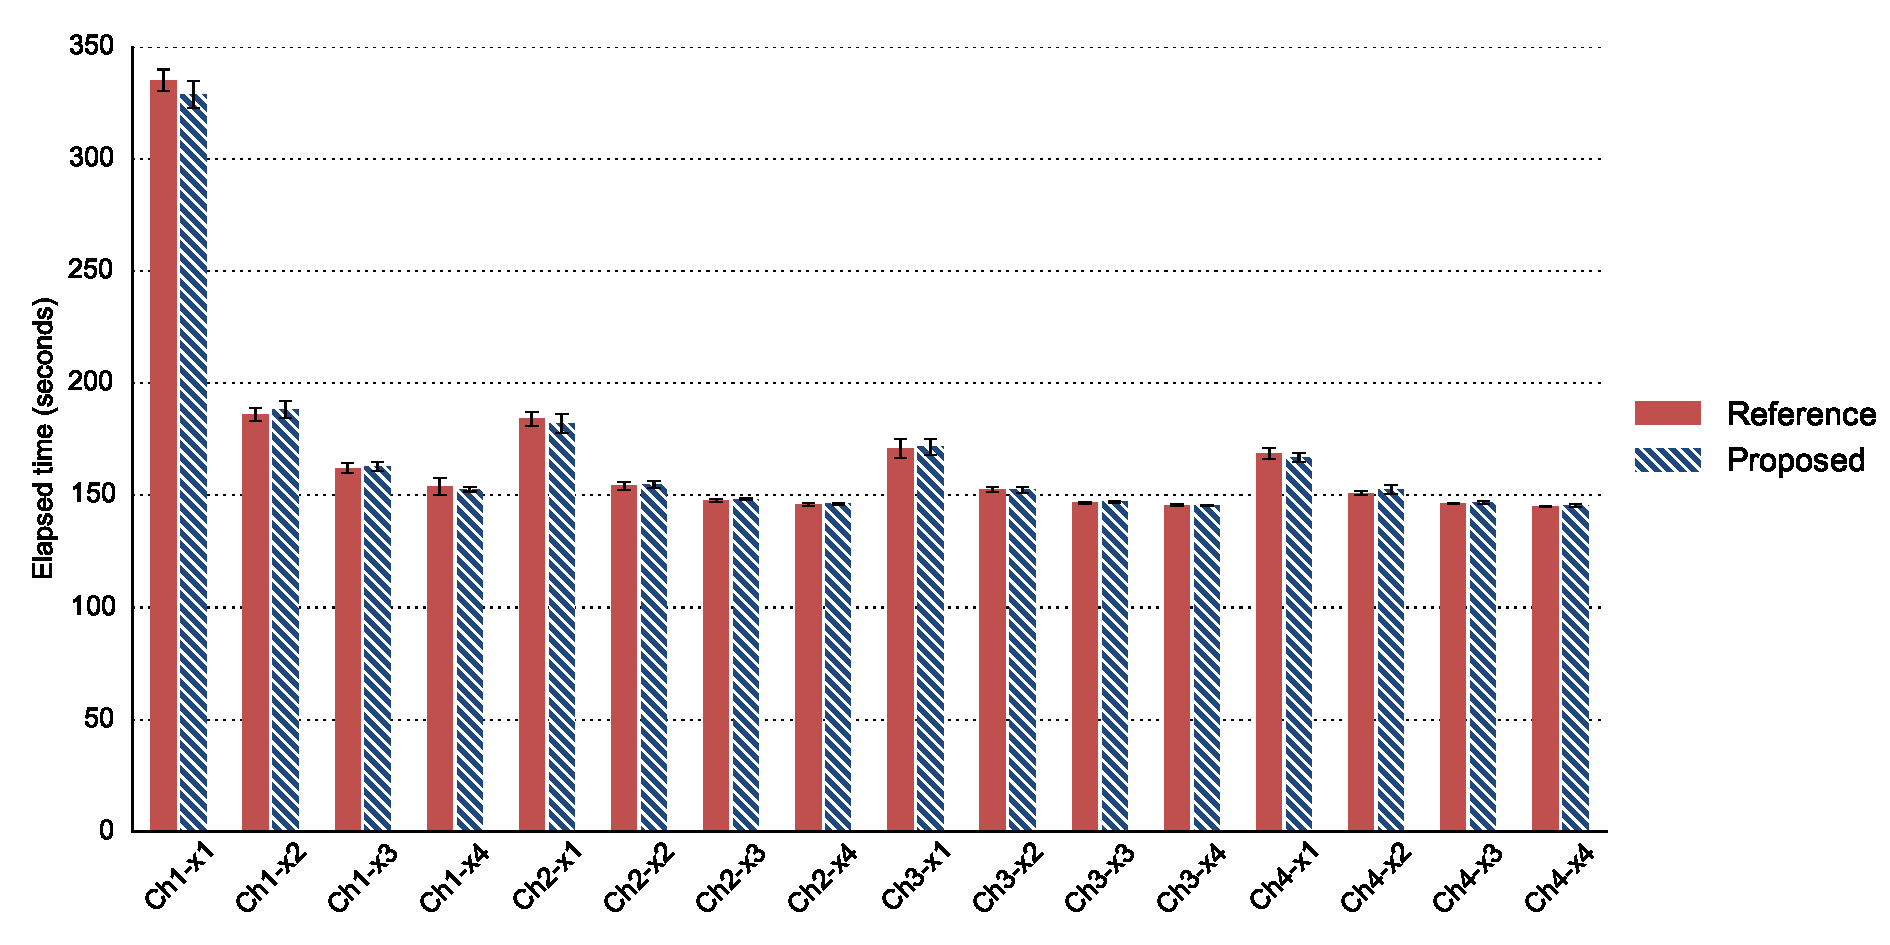
\includegraphics[width=\textwidth]{figures/ch6-fig-11.pdf}
	\caption[Elapsed time of Linux kernel source archive extraction and word count.]{\label{fig:ch6-fig-11}Elapsed time of Linux kernel source archive extraction and word count. Error bars represent the 95\% confidence intervals of the means.}
\end{figure}

\begin{table}[htbp]%
	\centering
	\caption{Frequency of disk model rollback operations for the Linux kernel source archive extraction and work count workload}\label{tab:ch6-7-rollback}
	\noindent\begin{tabular}{cc}
		\toprule
		Storage device configuration &
		Percentage of I/Os causing rollbacks \\
		\midrule
		Ch1-x1 & 0\% \\
		Ch1-x2 & 0\% \\
		Ch1-x3 & 0\% \\
		Ch1-x4 & 0\% \\
		Ch2-x1 & 96\% \\
		Ch2-x2 & 91\% \\
		Ch2-x3 & 87\% \\
		Ch2-x4 & 80\% \\
		Ch3-x1 & 97\% \\
		Ch3-x2 & 91\% \\
		Ch3-x3 & 85\% \\
		Ch3-x4 & 81\% \\
		Ch4-x1 & 95\% \\
		Ch4-x2 & 90\% \\
		Ch4-x3 & 86\% \\
		Ch4-x4 & 81\% \\
		\bottomrule
	\end{tabular}
\end{table}%

Besides using synthetic workloads, the proposed storage device emulator is also validated using real application programs. In this test, the ext4 file system is created on the emulated storage device and both scenarios for the NOOP I/O scheduler and the CFQ I/O scheduler are tested. The Linux kernel source archive (linux-3.10.tar.bz2) downloaded from kernel.org~\cite{Kernel:2013:3.10source} is first copied to the ext4 file system and then extracted in place. Table~\ref{tab:ch6-linux-archive} lists the information about the size and the number of files for the top level directories in the archive. The percentage of all the I/O requests that will cause disk model simulation time rollbacks are listed in Table~\ref{tab:ch6-7-rollback}  


\begin{table}[htbp]%
	\small
	\begin{center}
		\caption{Contents of the Linux kernel source archive}\label{tab:ch6-linux-archive}
		\noindent\begin{tabular}{lrr}
		\toprule

		Directory name & Content size & Number of files \\
		\midrule
		./init & 180KB & 13 \\
		./net & 23M & 1417 \\
		./Documentation & 24M & 2581 \\
		./samples & 204K & 34 \\
		./usr & 40K & 5 \\
		./ipc & 240K & 15 \\
		./arch & 126M & 15497 \\
		./virt & 216K & 14 \\
		./security & 2.2M & 169 \\
		./crypto & 2.5M & 113 \\
		./scripts & 2.7M & 250 \\
		./firmware & 6.0M & 151 \\
		./tools & 5.2M & 616 \\
		./block & 912K & 64 \\
		./fs & 35M & 1726 \\
		./sound & 26M & 1434 \\
		./kernel & 5.8M & 273 \\
		./drivers & 283M & 14824 \\
		./lib & 2.1M & 234 \\
		./include & 27M & 3493 \\
		./mm & 2.7M & 83 \\		
		\bottomrule
		\end{tabular}
	\end{center}
\end{table}%

Because the total size of the entire working set will be over 400MB, the contents under the Documentation and the drivers directories in the source archive are omitted. After extraction, the total number of words in the source files is then counted using the wc utility. The total elapsed time for extracting the kernel achieve and performing the word count is measured. All results from the proposed storage device emulator are within 2\% differences to the results from the reference system. The measured results for the CFQ I/O scheduler are listed in Table~\ref{tab:ch6-7} and graphed in Figure~\ref{fig:ch6-fig-11}.

This test scenario highlights a limitation of the reference local emulation type emulator: the size of the storage device that can be emulated is limited to the size of the available memory which can be used as the backing storage. In this test, the Documentation and the drivers directories in the kernel source archive need to be omitted so that the total working set will fit into the 400MB storage device. In comparison, the proposed storage device emulator does not have this kind of limitation. The size of the storage device that can be emulated by the proposed storage device emulator can be as large as the backing storage available on the emulator server. Moreover, because the state of the OS is paused while the backing storage is being accessed, the performance evaluation results will not be affected by the speed of the backing storage used. This means that slower backing storages can be used for emulating faster storage devices. In our experiments, the backing storage device used by the proposed storage device emulator is a traditional hard disk drive, and the proposed storage device emulator have no problem using it for emulating storage devices that have sub-millisecond response times.


\subsection{Video Encoding and Decoding}
\label{sec:ch6-6.6.4}

\begin{table}[htbp]%
	\small
	\begin{center}
	\caption[Elapsed time of MPEG2 video encoding and decoding]{Elapsed time of MPEG2 video encoding and decoding the CIF resolution \textit{foreman} sequence}\label{tab:ch6-8}
	\hspace*{-2cm}
	\noindent\begin{tabular}{
			l
			S[table-format=2.2]
			S[table-format=2.2]
			S[table-format=2.2]
			S[table-format=2.2]
			S[table-format=2.2]
			S[table-format=2.2]
			S[table-format=1.2]
			S[table-format=1.2]
			r}
		\toprule
		{Test Config} & {Mean} & {Median} & {Low} & {High} & {Min} & {Max} & {SDEV\%} & {HW\%} & \multicolumn{1}{c}{Diff} \\
		\midrule
		
Ch1-x1 Ref. & 12.48  & 12.55  & 12.33  & 12.64  & 12.22  & 12.83  & 1.76  & 1.26 & \\
Ch1-x1 & 12.57  & 12.64  & 12.39  & 12.74  & 12.23  & 12.84  & 1.94  & 1.39 & 0.67\% \\
Ch1-x2 Ref. & 8.56  & 8.56  & 8.49  & 8.63  & 8.43  & 8.68  & 1.14  & 0.82 & \\
Ch1-x2 & 8.56  & 8.54  & 8.50  & 8.62  & 8.47  & 8.69  & 0.97  & 0.70 & -0.06\% \\
Ch1-x3 Ref. & 7.22  & 7.24  & 7.20  & 7.25  & 7.15  & 7.27  & 0.55  & 0.39 & \\
Ch1-x3 & 7.22  & 7.23  & 7.16  & 7.27  & 7.09  & 7.36  & 1.07  & 0.77 & -0.10\% \\
Ch1-x4 Ref. & 6.72  & 6.68  & 6.66  & 6.77  & 6.64  & 6.83  & 1.12  & 0.80 & \\
Ch1-x4 & 6.66  & 6.66  & 6.63  & 6.69  & 6.59  & 6.71  & 0.62  & 0.44 & -0.83\% \\
Ch2-x1 Ref. & 8.98  & 8.98  & 8.83  & 9.14  & 8.47  & 9.28  & 2.48  & 1.77 & \\
Ch2-x1 & 8.94  & 8.93  & 8.75  & 9.14  & 8.44  & 9.32  & 3.07  & 2.20 & -0.47\% \\
Ch2-x2 Ref. & 7.00  & 7.02  & 6.92  & 7.09  & 6.78  & 7.21  & 1.77  & 1.26 & \\
Ch2-x2 & 6.91  & 6.94  & 6.80  & 7.01  & 6.69  & 7.15  & 2.11  & 1.51 & -1.38\% \\
Ch2-x3 Ref. & 6.48  & 6.50  & 6.44  & 6.53  & 6.37  & 6.56  & 0.94  & 0.67 & \\
Ch2-x3 & 6.48  & 6.47  & 6.42  & 6.53  & 6.35  & 6.57  & 1.10  & 0.79 & -0.14\% \\
Ch2-x4 Ref. & 6.31  & 6.32  & 6.29  & 6.34  & 6.26  & 6.36  & 0.51  & 0.37 & \\
Ch2-x4 & 6.32  & 6.31  & 6.29  & 6.35  & 6.25  & 6.38  & 0.63  & 0.45 & 0.08\% \\
Ch3-x1 Ref. & 8.08  & 8.11  & 7.89  & 8.28  & 7.58  & 8.69  & 4.02  & 2.43 & \\
Ch3-x1 & 8.14  & 8.10  & 7.94  & 8.33  & 7.69  & 8.76  & 3.93  & 2.37 & 0.67\% \\
Ch3-x2 Ref. & 6.80  & 6.80  & 6.76  & 6.85  & 6.68  & 6.87  & 0.95  & 0.68 & \\
Ch3-x2 & 6.79  & 6.80  & 6.72  & 6.87  & 6.58  & 6.92  & 1.51  & 1.08 & -0.15\% \\
Ch3-x3 Ref. & 6.40  & 6.40  & 6.37  & 6.43  & 6.30  & 6.47  & 0.72  & 0.52 & \\
Ch3-x3 & 6.39  & 6.37  & 6.35  & 6.42  & 6.31  & 6.44  & 0.71  & 0.51 & -0.20\% \\
Ch3-x4 Ref. & 6.23  & 6.23  & 6.21  & 6.25  & 6.17  & 6.27  & 0.48  & 0.34 & \\
Ch3-x4 & 6.22  & 6.24  & 6.18  & 6.26  & 6.09  & 6.30  & 0.91  & 0.65 & -0.11\% \\
Ch4-x1 Ref. & 7.84  & 7.84  & 7.73  & 7.95  & 7.65  & 8.09  & 1.91  & 1.37 & \\
Ch4-x1 & 7.83  & 7.87  & 7.65  & 8.01  & 7.22  & 8.18  & 3.63  & 2.31 & -0.15\% \\
Ch4-x2 Ref. & 6.69  & 6.70  & 6.65  & 6.73  & 6.61  & 6.77  & 0.82  & 0.58 & \\
Ch4-x2 & 6.63  & 6.61  & 6.57  & 6.69  & 6.51  & 6.74  & 1.19  & 0.85 & -0.88\% \\
Ch4-x3 Ref. & 6.33  & 6.33  & 6.31  & 6.35  & 6.29  & 6.37  & 0.45  & 0.32 & \\
Ch4-x3 & 6.34  & 6.35  & 6.30  & 6.38  & 6.25  & 6.41  & 0.83  & 0.59 & 0.11\% \\
Ch4-x4 Ref. & 6.14  & 6.15  & 6.12  & 6.15  & 6.10  & 6.16  & 0.36  & 0.26 & \\
Ch4-x4 & 6.17  & 6.18  & 6.15  & 6.19  & 6.10  & 6.20  & 0.45  & 0.32 & 0.57\% \\

		\bottomrule
	\end{tabular}
	\hspace*{-2cm}
	\end{center}
	
	Remarks: Units are in seconds. Low and high are the Student-\textit{t} confidence interval error bar values. SDEV\% and HW\% are the standard deviation and half-width of the confidence interval as a percent of the mean.
\end{table}%

\begin{figure}[htpb]
	\centering
	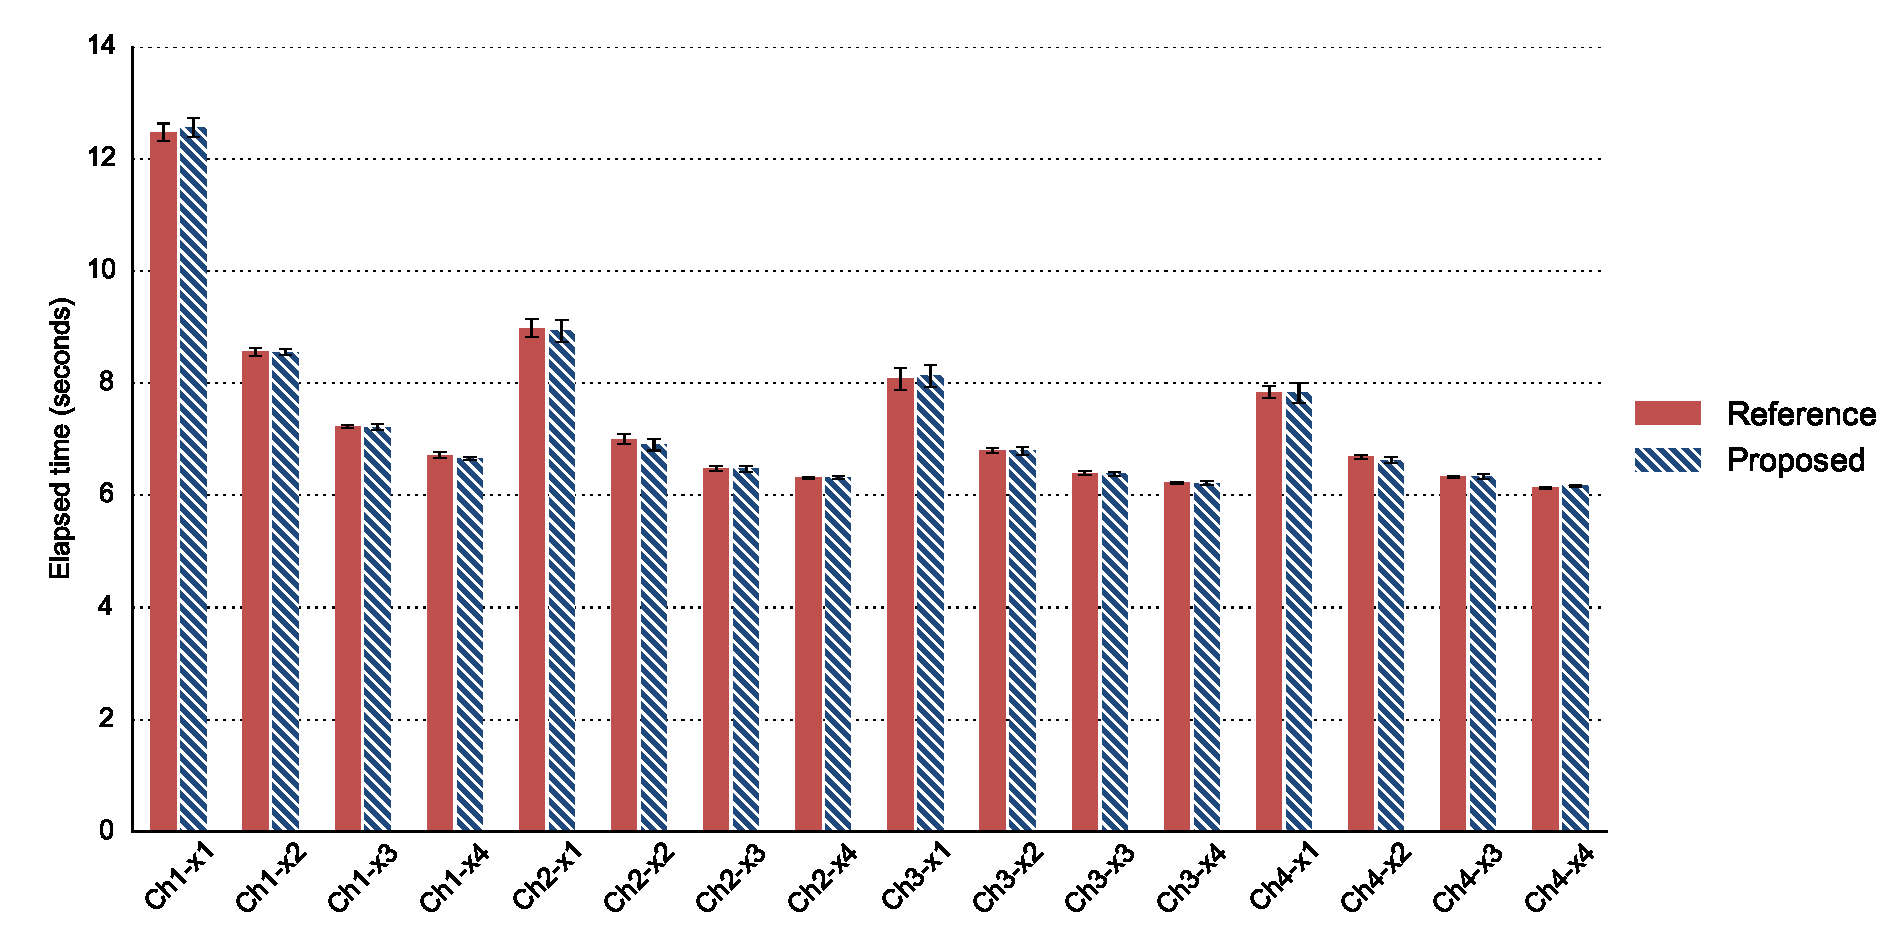
\includegraphics[width=\textwidth]{figures/ch6-fig-12.pdf}
	\caption[Elapsed time of MPEG2 video encoding and decoding.]{\label{fig:ch6-fig-12}Elapsed time of MPEG2 video encoding and decoding the CIF resolution \textit{foreman} sequence. Error bars represent the 95\% confidence intervals of the means.}
\end{figure}

\begin{table}[htbp]%
	\centering
	\caption{Frequency of disk model rollback operations for the MPEG2 video encoding and decoding workload}\label{tab:ch6-8-rollback}
	\noindent\begin{tabular}{cc}
		\toprule
		Storage device configuration &
		Percentage of I/Os causing rollbacks \\
		\midrule
		Ch1-x1 & 0\% \\
		Ch1-x2 & 0\% \\
		Ch1-x3 & 0\% \\
		Ch1-x4 & 0\% \\
		Ch2-x1 & 76\% \\
		Ch2-x2 & 72\% \\
		Ch2-x3 & 75\% \\
		Ch2-x4 & 74\% \\
		Ch3-x1 & 75\% \\
		Ch3-x2 & 75\% \\
		Ch3-x3 & 75\% \\
		Ch3-x4 & 73\% \\
		Ch4-x1 & 74\% \\
		Ch4-x2 & 78\% \\
		Ch4-x3 & 74\% \\
		Ch4-x4 & 73\% \\
		\bottomrule
	\end{tabular}
\end{table}%

In this test, the ext3 file system is created on the emulated storage device and both scenarios for the NOOP I/O scheduler and the CFQ I/O scheduler are tested. In the test, the raw CIF resolution \textit{foreman} video sequence is first copied to the ext3 file system. The raw video sequence is then encoded to the MPEG2 format using the \textit{avconv}~\cite{Libav:2014} video encoder. After encoding, the encoded MPEG2 sequence is decoded back to the raw format using the \textit{avconv} video decoder. The total elapsed time for encoding and decoding the video sequence is measured. All results from the proposed storage device emulator are within 2\% differences to the results from the reference system. The measured results are listed in Table~\ref{tab:ch6-8} and graphed in Figure~\ref{fig:ch6-fig-12}. The percentage of all the I/O requests that will cause disk model simulation time rollbacks are listed in Table~\ref{tab:ch6-8-rollback}

\subsection{Effects of Disk Model Complexity on Conventional Storage Device Emulators}

One problem with the conventional storage device emulators is that if the time it takes to simulate the disk model exceeds the response times of the corresponding I/O request, then the emulator will fail to emulate the intended behavior of the target storage device. For example, if it takes the emulator 2\si{\milli\second} to simulate the disk model for an I/O response, then the emulator will inevitably fail to properly emulate I/O responses that are supposed to be completed faster than 2\si{\milli\second}. The faster the storage device is, the more likely that the emulator will fail to emulate the correct response timings for the I/O requests. In this section, we evaluate how the amount of time needed for simulating the disk model can affect the local emulation type emulator used in the reference system.

To get a sense of how much time that a typical disk model simulator would require for simulating an I/O request, we ported the DiskSim simulator version 4.0~\cite{Bucy:2008} to ZedBoard and measured its operation speed. In our measurement, it took DiskSim approximately 37 seconds to simulate 10,000 I/O operations for a disk device. That is, the amount of time required for simulating each I/O request is about 3.7\si{\milli\second}.

To study the effect of disk model complexity on the conventional storage device emulators, we introduce artificial delays to the disk model used by the reference system to simulate disk models of different complexity. The timing delays introduced to the disk model are ranged from 0.25\si{\milli\second} to 2\si{\milli\second} in 0.25\si{\milli\second} increments. The sequential read bandwidth benchmark described in section~\ref{sec:ch6-6.6.1} is used for testing. The evaluation results are illustrated in Figure~\ref{fig:ch6-fig-13}. To save space, only the results for the single channel storage device configurations are shown. From the results, we can see that the faster the emulated storage device is, the more impact that disk model complexity will have on the reference system. For example, when emulating faster storage devices, such as the storage device with the Ch1-x4 configuration, even a disk model processing time of just 1\si{\milli\second} can affect the predicted performance by more than 50\%.

\begin{figure}[htpb]
	\centering
	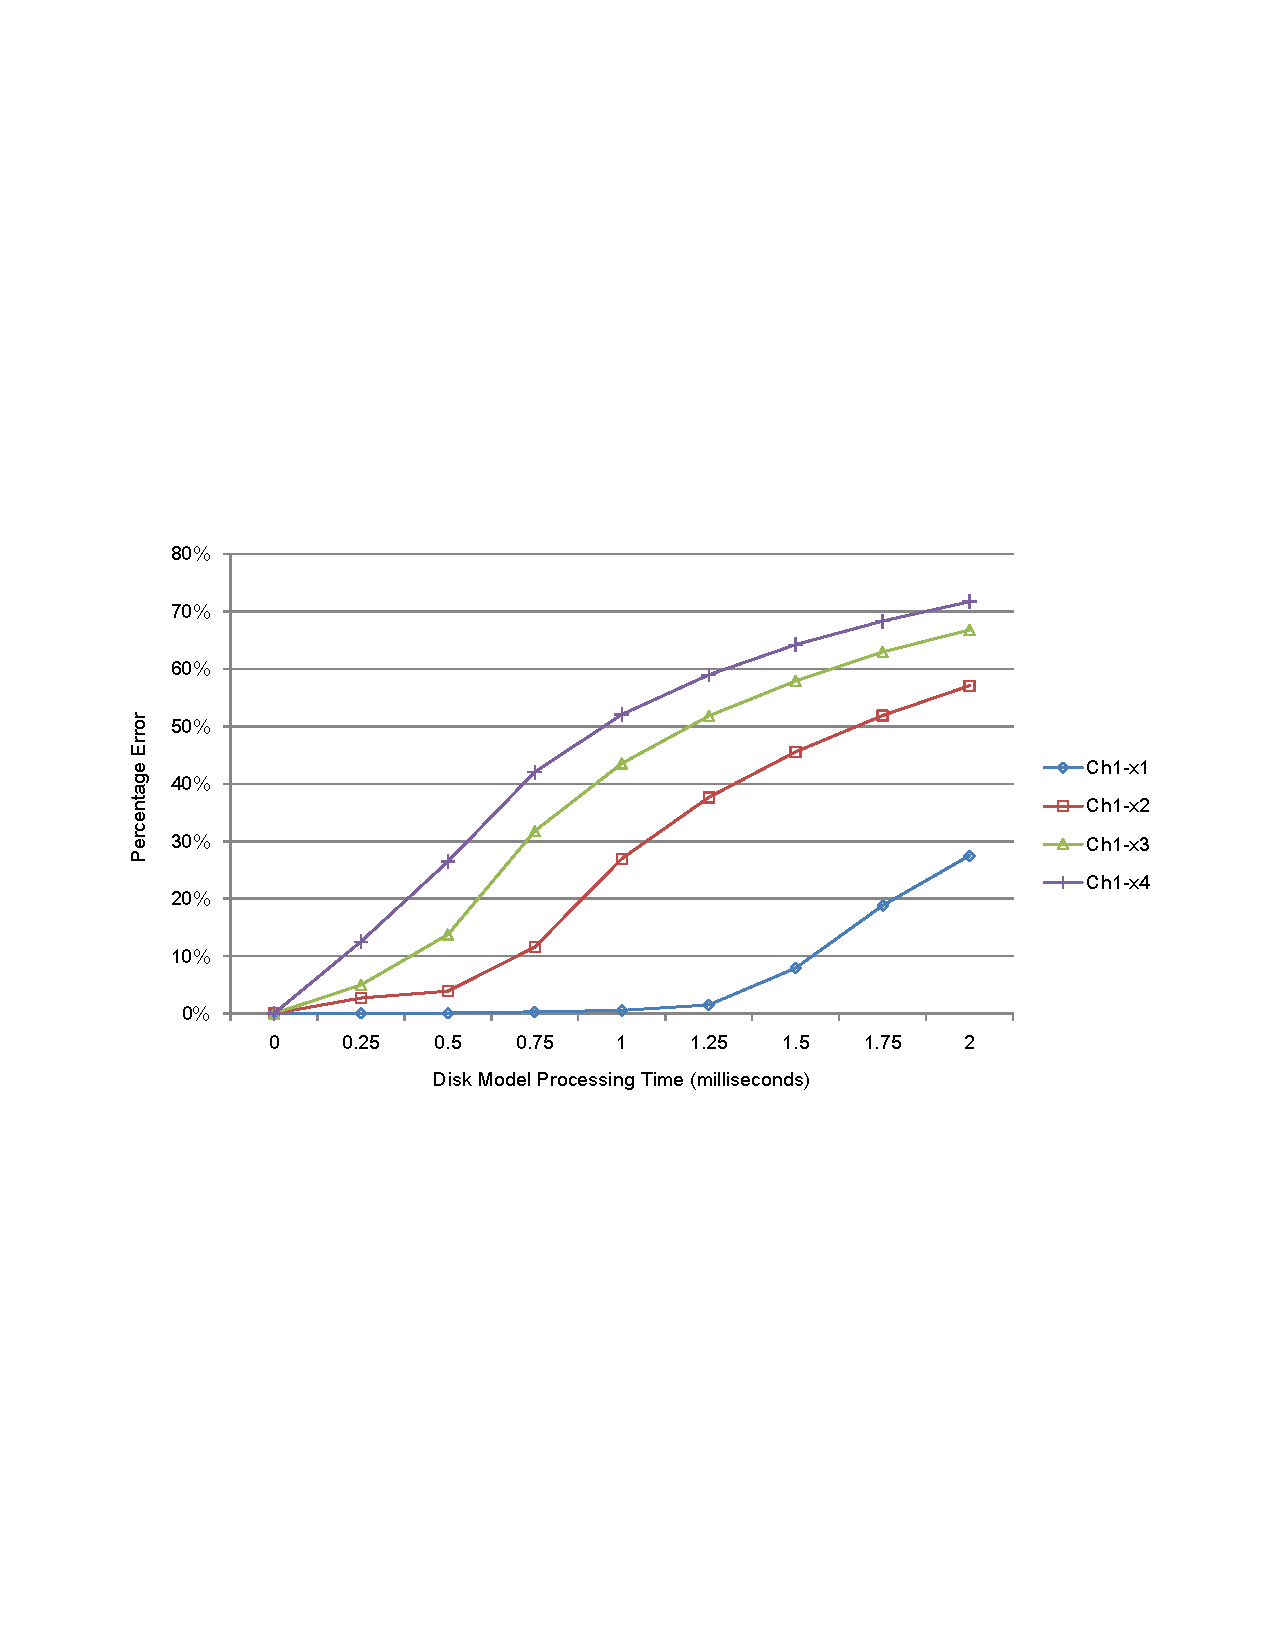
\includegraphics[trim=2cm 9.2cm 2cm 9cm, width=\textwidth]{figures/ch6-fig-13.pdf}
	\caption[Effects of disk model processing time on conventional storage device emulators.]{\label{fig:ch6-fig-13}Effects of disk model processing time on conventional storage device emulators. In conventional storage device emulators, disk model processing time can affect the characteristics of the emulated storage device and thus lead to performance evaluation errors.}
\end{figure}

In comparison, in the proposed emulator, because the OS is put into the paused state while the emulator server is simulating the disk model, the evaluation results from the proposed emulator will not be affected by the complexity of the disk model. This means that disk models of arbitrary complexity can be used in the proposed emulator for modeling complex storage device behaviors.